\documentclass[12pt, a4paper, oneside]{report}

\usepackage{mathptmx}        
\usepackage[scaled=0.92]{helvet}
\usepackage{courier}
\usepackage{minted}
\usepackage{setspace}
\onehalfspacing

\usepackage{geometry}
\geometry{a4paper, margin=1in}

\usepackage{graphicx}
\usepackage{caption}
\usepackage{amsmath, amssymb, siunitx}
\usepackage{parskip}
\usepackage{fancyhdr}
\usepackage{booktabs}

\usepackage{titlesec}
\titleformat{\chapter}{\normalfont\Huge\bfseries}{\thechapter.}{1em}{}
\titlespacing*{\chapter}{0pt}{-30pt}{10pt}

\pagestyle{fancy}
\fancyhf{}
\cfoot{\thepage}
\renewcommand{\headrulewidth}{0pt}

\usepackage[colorlinks=true, linkcolor=black, citecolor=black, urlcolor=blue]{hyperref}

\begin{document}

\pagenumbering{gobble}

\begin{center}
    \vspace*{0.8cm}
    
    \Large \textbf{Quantum Inspired Vision-Language: A Tensorial Approach} \\

        
    \vspace{0.8cm}
    
    \large \textbf{Fotinos Kyriakides} \\
    \large Supervisor: Mehrnoosh Sadrzadeh \\
    \vspace{0.2cm}
    
    
    \large University College London \\
    \vspace{0.2cm}
    
    
    % \rule{\textwidth}{0.4pt}
    
    \large \textbf{Abstract}
    \end{center}
        
\normalsize

% TODO: shorten this - 200 words max

Tensor networks are a natural quantum-native architecture for image encoding, since their contraction structure mirrors the spatial hierarchy of an image. Several candidate architectures exist, but their relative merits under NISQ constraints have not been established empirically.

We investigate a family of quantum image encoders spanning tree, matrix-product and MERA topologies, and narrow within the surviving topology across four data encodings, three variational ansätze and two readout protocols. Selection is driven by measured gradient variance as a function of qubit count, the information bandwidth of the readout, parameter efficiency, and the memory cost of classical simulation.

The selected architecture is a coherent quantum tree tensor network, in which image patches are encoded on qubits and contracted hierarchically through entangling unitaries, with intermediate states passed between levels as qubits rather than measured. It is trained in noiseless simulation at the largest resolution that remains tractable.

We evaluate on CLEVR against classical tensor-network and neural baselines. The quantum tower exceeds its direct classical analogue, the same tree with CP-decomposed nodes in place of unitaries, on shape classification while carrying 18\% fewer parameters, with parity on the remaining three attributes; an unstructured neural baseline of roughly twice the size leads on every attribute. The unitarity constraint therefore does not reduce representational capacity at this scale, though hierarchical contraction does not by itself close the gap to an unstructured network on perception. A variant carrying no positional parameters attains parity on spatial-relation classification, establishing that the tree topology encodes position implicitly. On a binding task with class-conditional marginals equalised by construction, where every classical architecture falls to chance under patch shuffling, classical tensor networks reach 91–93\% and a parameter-matched MLP 94.6\%; the quantum tree, carrying no positional parameters at all, separates the arrangements on 5 of 15 initialisations and peaks 8.1 standard deviations above chance.

Substituting a tensor-network vision tower for frozen CLIP yields a vision-language model that is quantum-inspired end to end. On ARO, this model improves attribution accuracy from 70\% to 77.65\% and relation accuracy from 55.81\% to 59.78\%.
    
    
\newpage

\tableofcontents
\newpage

\chapter*{Acknowledgement and Statement of Contribution}

I would like to thank my supervisor Professor Mehrnoosh Sadrzadeh for her continuous help and guidance throughout this  project. I would also like to acknowledge the work of the Quantum Learning UCL group for their help in developing this work, for engaging in interesting discussions, providing ideas and scrutinizing the generated results. 
This line of work runs parallel to theirs in multiple ways, with the initial goal of finding a quantum inspired image model, being directly linked to their previous work on a quantum inspired text model (DisCoCat). Additionally, the quantum image model implementation run parallel to their implementation of the text model, with many fruitful conversations of promising areas of exploration, such as data reuploading as a quantum counterpart to residuals. 



\newpage

% =============================================
% 4. INTRODUCTION
% =============================================
\pagenumbering{arabic}  
\setcounter{page}{1}

\chapter{Introduction}
% An introductory section, which states the aims and objectives of the project, discusses the rationale for the project (including how it relates to previous work), and outlines what is covered by each main section in the report.

% \section{Aims and Objectives}
% [State the specific goals of your project. Use bullet points or a numbered list.]

% \section{Rationale and Previous Work}
% [Discuss why this project matters. Link to previous research with citations.]

% \section{Report Outline}
% [Briefly describe what each chapter covers. End with: "Chapter 2 covers the 
% methodology. Chapter 3 presents the results. Chapter 4 discusses the findings 
% and concludes."]

Quantum machine learning models promise large improvements over classical ones in both parameter count and expressiveness by taking advantage of quantum effects like entanglement and superposition. These advantages however come at a cost; some arise due to the computational limitations of the NISQ era \cite{nisq}, while others are intrinsic to the quantum paradigm.

In this work, we set off to explore possible architectures for a quantum-inspired image encoder. The field of quantum-inspired machine learning \cite{quantum_inspired} mostly revolves around using tensor network architectures. This framework allows for both a classical and a quantum model to be developed in parallel, an approach we adopt in this work. We explore how classical features, like dropout \cite{dropout} and residual connections \cite{residuals}, can be applied to quantum circuits and whether or not they are needed. Moreover, we investigate how the selection of ansätze and encoding methods affects the expressivity of the model, its depth and parameter efficiency.

Beyond architectural details, we evaluate and contrast the resulting tensor network's performance with contemporary MLP models on various benchmarks across perception, relation, and composition tasks. 
% In doing so, we report two core findings regarding the vision tower: first, that the unitarity-constrained quantum node achieves higher parameter efficiency than its unconstrained classical counterpart, and second, that within the vision tower itself, tensor networks show no compositional advantage over a parameter-matched MLP.

As a secondary objective, we explore how this architecture performs within a broader multimodal context. Contemporary Vision Language Models (VLMs) heavily rely on contrastive learning architectures\cite{clip} that frequently exhibit "bag-of-words" behavior, struggling on compositional benchmarks that require a strict understanding of spatial layout \cite{aro}. By combining our classical quantum-inspired image model with an existing quantum-inspired text model, we yield the first fully quantum-inspired vision-language model. 
% Evaluating this integrated model reveals our third finding: that the baseline frozen CLIP encoder is measurably blind to compositional binding, discarding spatial information that the smaller models readily capture.

Ultimately, the aims of this project are threefold: (i) to explore viable quantum-inspired image encoder architectures using tensor networks; (ii) to rigorously benchmark the parameter efficiency and compositional capabilities of the quantum unitary node against classical unconstrained nodes and MLPs; and (iii) to integrate this image encoder into a multimodal framework to assess whether a structurally rigorous architecture can overcome the compositional limitations of standard contrastive VLMs.

\chapter{Related Work}

\section{Language}
Historically, natural language processing has struggled to balance the continuous semantic representation of individual words with the strict structural rules that bind them together. Early approaches, such as Bag-of-Words \cite{bow} and TF-IDF \cite{tfidf}, prioritized vocabulary presence over structure, representing text purely by word frequency. While computationally cheap, these methods completely fail at compositionality; they yield identical representations for "the man biting the dog" and "the dog biting the man". The subsequent introduction of static word embeddings like Word2Vec \cite{word2vec} and GloVe \cite{glove} successfully captured distributional semantics, mapping words to dense vectors where spatial distance denotes semantic similarity. However, composing full sentences typically relied on rudimentary operations like vector addition or averaging, flattening the text and destroying the hierarchical grammar necessary for complex relational meaning.

To capture word order, sequential architectures like Recurrent Neural Networks (RNNs) \cite{rnn} and Long Short-Term Memory (LSTM) \cite{lstm} networks were introduced. While these models capture the one-dimensional sequential nature of text, they create a severe information bottleneck by compressing an arbitrarily long sentence into a single, fixed-size hidden state. Furthermore, they process text strictly from left to right rather than relationally, failing to inherently model the hierarchical tree structures of human language. This bottleneck was bypassed by the Transformer architecture \cite{attention}, which discarded recurrence entirely in favor of parallelized global self-attention. However, self-attention introduces a different compositional failure: it treats the input sequence as a fully connected graph rather than a strict linguistic hierarchy. Lacking built-in relational rules for syntax, Transformers are forced to simulate compositionality by scaling up to massive parameter counts and relying on vast amounts of training data.

In contrast to these bottom-up, data-driven approaches, computational linguistics offers a top-down paradigm that guarantees structural hierarchy by design. The Categorical Compositional Distributional (DisCoCat) model \cite{discocat} provided a foundational breakthrough by mathematically unifying continuous distributional semantics with formal, rigorous compositional logic trees. Grounded in applied category theory, DisCoCat maps the syntactic types of Pregroup algebra \cite{pregroup} directly onto continuous vector spaces. In this framework, words are no longer uniform vectors; their tensor order is strictly dictated by their grammatical function. A noun is represented as a standard 1D vector, while a transitive verb acts as a 3rd-order tensor. The holistic meaning of a sentence is computed deterministically by contracting these constituent tensors along their shared grammatical indices.

While this achieves native, mathematically rigorous text compositionality, representing functional words as high-order tensors introduces severe dimensional scaling that is classically intractable. To resolve this, DisCoCat borrows mathematical engines from many-body quantum physics, specifically Matrix Product States (MPS) \cite{mps_physics}. Just as MPS factorizes an exponentially large global quantum state into a 1D chain of manageable local tensors, it can be used to compress the massive tensor contractions of a DisCoCat sentence. By substituting quantum entanglement bonds with Pregroup grammatical dependencies, MPS provides a highly parameter-efficient, structurally rigorous language architecture that successfully resolves the compositionality bottleneck for text.

\section{Vision}

Computer vision models have historically struggled to capture precise part-whole structural relationships, often settling for a "bag of features" approach rather than achieving true compositional understanding. Early Multi-Layer Perceptrons (MLPs) \cite{mlp} treated images as unstructured data, requiring a deterministic flattening into a 1D vector that inherently destroyed the 2D topological structure and spatial proximity of the pixels. Convolutional Neural Networks (CNNs) \cite{cnn} addressed this by introducing local receptive fields to extract hierarchical features. However, to manage dimensionality, CNNs rely heavily on downsampling mechanisms like max-pooling. While pooling introduces translation invariance, it discards the precise relative positions of features within the pooling window. This spatial invariance causes CNNs to act as a loose collection of local features, failing at rigorous part-whole compositional tasks (the "Picasso effect", where a CNN might classify a face even if the features are spatially scrambled).

To bypass the limitations of convolutions, the Vision Transformer (ViT) \cite{vit} adapted the NLP self-attention mechanism for image data. A ViT divides an image into a sequence of flattened patches and applies global self-attention. Because this operation treats the input as a 1D sequence of tokens, the ViT completely discards the native 2D grid inductive bias, relying entirely on learned positional embeddings to retain spatial context. Much like text Transformers, ViTs lack built-in relational rules for 2D data. By treating image patches as a fully connected graph, they are forced to brute-force the understanding of spatial relationships through massive parameter counts and vast datasets.

In the multimodal domain, the evolution of Vision Language Models (VLMs) has centered on mapping these visual representations to language. Early architectures, such as ViLBERT \cite{vilbert} and LXMERT \cite{lxmert}, relied on computationally heavy pipelines using off-the-shelf object detectors to extract bounding boxes. This bounded the models to predefined vocabularies and destroyed the holistic 2D spatial context of the image. A paradigm shift occurred with the introduction of OpenAI's CLIP \cite{clip}, which eliminated bounding boxes in favor of aligning independent text and image encoders using a global contrastive InfoNCE loss \cite{infonce}. While highly scalable, this global alignment introduces a fatal flaw: the vision "bag-of-words" problem \cite{aro}. Because CLIP relies entirely on global feature alignment without any inherent structural inductive bias, it maps global visual features to global text vocabulary while remaining functionally blind to syntax and spatial layout. Consequently, the model fails to distinguish between text like "a glass on a table" and "a table on a glass", performing at near-chance levels on compositional benchmarks.

This asymmetry between rigorous compositional text models and non-hierarchical vision models is perfectly encapsulated by the DisCoClip baseline \cite{discoclip}. DisCoClip successfully extended the DisCoCat language framework into a multimodal setting by grafting it onto a frozen CLIP vision backbone. While this provided a highly parameter-efficient and structurally rigorous text engine, the framework's end-to-end compositional reasoning was ultimately bottlenecked by CLIP's spatial limitations. To achieve true relational understanding, the spatially invariant vision encoder must be replaced with an architecture that inherently preserves 2D compositional hierarchies.

Quantum-inspired tensor networks provide this capability. While 1D Tensor Trains (TT) destructively flatten images and 2D Projected Entangled Pair States (PEPS) are computationally intractable (P-complete), Tree Tensor Networks (TTNs) \cite{ttn_images} emerge as the optimal topology. By recursively contracting patches of pixels into a pyramid-like structure, a TTN maintains a manageable computational footprint while natively capturing and preserving high-level relational features and 2D spatial hierarchies.

\section{Quantum Tensor Networks and VQCs}

While tensor networks, such as the Matrix Product States used in NLP and the Tree Tensor Networks adapted for vision, provide mathematically rigorous solutions to the compositionality bottleneck in classical machine learning, their origins lie in many-body quantum physics \cite{mps_physics}. Because they were fundamentally designed to model quantum entanglement, tensor networks possess a native correspondence with quantum computing.

In a classical tensor network, each node applies an unconstrained mathematical operation (such as a CP-decomposition) to contract its inputs. However, if this contraction is constrained to be a unitary operation ($U^{\dagger}U=I$), the tensor network maps directly onto a Variational Quantum Circuit (VQC). For hierarchical architectures, this structural equivalence, the TTN $\leftrightarrow$ VQC correspondence, allows a classical vision architecture to be transpiled natively into a quantum circuit, where classical tensor contractions are replaced by unitary rotations and entanglement gates on qubits.

Consequently, this provides a rare opportunity to evaluate the exact same architectural topology across both classical and quantum paradigms. By comparing an unconstrained classical tensor network against a unitary-constrained quantum circuit, we can rigorously isolate the effect of the quantum paradigm on parameter efficiency and expressive capacity, answering whether the unitary constraint acts as a handicap or a powerful structural regularizer.

% \section{Report Outline}

\chapter{Theoretical Framework and Candidate Architectures}
\label{ch:theory}

\section{Universal Quantum Circuit Mechanics}

Unlike classical neural networks, which natively process and propagate continuous real-valued matrices, quantum machine learning models operate exclusively within a complex Hilbert space. As a result, all quantum machine learning models operating on classical data need to select a way to encode this information onto quantum states as well as the foundational components of the variational quantum circuits.

\subsection{Data Encoding Strategies}
Before quantum computation can occur, classical information must be deterministically mapped into a quantum state. This dictates how effectively the model can utilize the Hilbert space.

\subsubsection{Amplitude Encoding}
Amplitude Encoding \cite{amplitude_encoding} maps an entire vector of normalized classical data $\mathbf{x} \in \mathbb{R}^{2^N}$ directly into the complex amplitudes of an $N$-qubit quantum state:
\begin{equation}
    |\psi(\mathbf{x})\rangle = \sum_{i=0}^{2^N-1} x_i |i\rangle \quad \text{where} \quad \sum |x_i|^2 = 1
\end{equation}
While this provides an optimal, exponential compression of classical data into the quantum Hilbert space, its physical implementation requires deep, dense circuits that are often prohibitively difficult to train and execute on NISQ devices.

\subsubsection{Scalar Rotation Encoding (\texttt{scalar\_ry})}
\label{sec:enc_scalar_ry}
An alternative is angle embedding \cite{angle_embedding}, which embeds a classical data point $x_i$ into the amplitude of a single qubit state by applying a Pauli-Y rotation:
\begin{equation}
    |\psi(x_i)\rangle = R_y(x_i) |0\rangle = \cos\left(\frac{x_i}{2}\right)|0\rangle + \sin\left(\frac{x_i}{2}\right)|1\rangle
\end{equation}
While highly gate-efficient and NISQ-friendly, this approach confines the encoded state strictly to a single plane of the Bloch sphere, significantly underutilizing the qubit's available state space. This encoding is referred to as \texttt{scalar\_ry} throughout; it appears under the alias \texttt{angle} in the single-node survey code, where it denotes the identical circuit.

\subsubsection{Multi-Axis Encoding (\texttt{multi\_axis})}
\label{sec:enc_multi_axis}
To increase representational capacity without increasing the qubit count, we evaluate a multi-axis encoding strategy \cite{data_reuploading}. This approach distributes the classical feature across multiple rotational axes sequentially:
\begin{equation}
    |\psi(x_i)\rangle = R_z(x_i) R_y(x_i) R_x(x_i) |0\rangle
\end{equation}
By explicitly maximizing the utilization of the Bloch sphere, multi-axis encoding embeds the classical data into a richer, more complex initial quantum state prior to entanglement.

\subsubsection{Second-Order Pauli-Z Feature Map (\texttt{zz\_map})}
\label{sec:enc_zz_map}
The three strategies above are all product encodings: each classical feature is written onto its own qubit independently, so the encoded state carries no correlation between features before the ansatz acts. To test whether entangling the data \textit{at encoding time} is worthwhile, we additionally evaluate the second-order Pauli-Z feature map of Havlíček et al.\ \cite{havlicek2019}. Hadamards prepare a uniform superposition, single-qubit $R_z$ rotations write each feature, and a ring of $ZZ$ couplings writes the pairwise products:
\begin{equation}
    |\psi(\mathbf{x})\rangle = \left[ \prod_{i} \text{IsingZZ}\big(x_i x_{i+1}\big) \right] \left[ \bigotimes_{i} R_z(x_i) \right] H^{\otimes N} |0\rangle^{\otimes N}
\end{equation}
where the product runs over adjacent wire pairs on a ring. The resulting state is entangled before the variational layer is applied, which raises the expressibility of the embedding but also makes it the most gate-expensive of the four.
\subsection{Parameterized Ansatz Design}
\label{sec:ansatz_design}
Once the data is encoded, the node must process it to extract relational features. This is achieved by applying a parameterized unitary operation $U(\theta)$, known as the ansatz. The structural design of the ansatz acts as the model's inductive bias.
\subsubsection{Hardware Efficient Ansatz (HEA)}
A standard baseline in variational quantum machine learning is the Hardware Efficient Ansatz (HEA) \cite{kandala2017}. This architecture applies successive layers of arbitrary single-qubit rotations followed by heavily connected entanglement gates (such as a ring of CNOTs). The unitary for a single layer $l$ operating on $N$ qubits is expressed as:
\begin{equation}
    U_{HEA}(\theta_l) = W_{ent} \prod_{j=1}^N R(\theta_{j,l})
\end{equation}
where $R$ represents parameterized $SU(2)$ rotations and $W_{ent}$ is the multi-qubit entangling array. While incredibly expressive, deep HEA circuits are famously susceptible to barren plateaus, where the variance of the gradient vanishes exponentially.

Two concrete instantiations of this family appear in the experiments that follow, and the distinction matters when reading the results tables. The broad single-node survey uses a \textit{star-entangler} variant, in which an $R_z$--$R_y$--$R_z$ rotation triple on each wire is followed by CNOTs from every child wire onto a single parent wire; this is the arm labelled \texttt{hea}. The ranked hybrid-tree evaluation instead uses PennyLane's \texttt{StronglyEntanglingLayers}, the canonical ring-entangler realisation, and is the arm labelled \texttt{strongly\_entangling}. Both are hardware-efficient in the sense defined above and differ only in entanglement topology; they are not the same circuit, and the two labels are not interchangeable.
\subsubsection{Alternating Layered Ansatz (ALT)}
To reduce the CNOT gate depth and explore different trainability profiles, we evaluate an Alternating Layered Ansatz (ALT). This architecture applies layers of parameterized Pauli-Y rotations followed by a "brickwork" entanglement structure, where CNOT gates alternate their connectivity at each layer (e.g., coupling even pairs in layer $l$, and odd pairs in layer $l+1$):
\begin{equation}
    U_{ALT}(\theta_l) = W_{brickwork}^{(l)} \prod_{j=1}^N R_y(\theta_{j,l})
\end{equation}
By restricting the rotation to a single axis and alternating the entanglement topology, ALT aims to maintain relational capacity while operating with a shallower, more noise-resilient circuit depth than HEA.
\subsubsection{Instantaneous Quantum Polynomial (IQP) Ansatz}
To strictly mitigate barren plateaus while preserving relational capacity, we evaluate the Instantaneous Quantum Polynomial (IQP) ansatz \cite{iqp_ansatz, havlicek2019}. Consisting of Hadamard gates flanking a diagonal parameterized unitary $D(\theta)$, the circuit is highly structured:
\begin{equation}
    U_{IQP}(\theta) = H^{\otimes N} D(\theta) H^{\otimes N}
\end{equation}
where $D(\theta)$ is typically an Ising-like Hamiltonian consisting of $Z$ rotations and $ZZ$ coupling gates. Because the core operations commute and are diagonal in the computational basis, the IQP ansatz possesses a strict, non-arbitrary inductive bias that alters the optimization landscape compared to HEA architectures.


\section{Candidate Architectures}
To rigorously isolate the effects of the quantum unitary constraint on parameter efficiency and expressive capacity, we constructed three topologically matched arms alongside a non-hierarchical task-difficulty baseline.

\subsection{The Quantum Coherent Tree (QTTN)}
The primary architecture under investigation is the Quantum Tree Tensor Network (QTTN). It operates on a 16-qubit device structured as a hierarchical quad-tree: 16 image patches are encoded into the leaves, contracted into 4 parent nodes, and finally contracted into a single root. The qubit count is set by the number of \textit{patches}, not by the image resolution: the input is always divided into a $4 \times 4$ grid, so a larger image yields larger patches rather than more qubits, and the circuit width is unchanged. Resolution therefore scales the classical patch-embedding layer that produces the rotation angles, while the simulation cost --- which is what binds here --- depends only on the 16 wires. The network applies parameterized unitary gates at each node. Because quantum evolution mandates that $U^\dagger U = I$, this architecture provides a naturally constrained, parameter-efficient framework. The QTTN serves as our core testbed to determine if structural quantum inductive biases can learn visual hierarchies.

\subsection{The Classical Control (CP-TTN)}
To answer whether the quantum unitary constraint helps or harms expressive capacity, we constructed a structurally faithful classical analogue: the \texttt{classical\_bare} model. This model shares the exact same 16-to-4-to-1 quad-tree topology as the QTTN, but replaces the unitary quantum nodes with unconstrained classical Canonical Polyadic (CP)\cite{cp_decomposition} tensor contractions. By matching the topology and sweeping the CP rank to bound the parameter budget, we can directly compare classical unconstrained capacity against quantum constrained capacity.

\subsection{The Classical Full Model}
While the \texttt{classical\_bare} arm matches the quantum constraints, standard classical architectures typically employ mechanisms like residual connections and dropout to prevent overfitting and vanishing gradients. The quantum equivalents of these components are evaluated. We introduced a \texttt{classical\_full} arm that includes them to quantify exactly how much of a performance gap is attributable to these standard classical regularizers.

\subsection{The MLP Reference}
A critical requirement for interpretability is calibrating task difficulty. We introduced a standard, non-hierarchical Multi-Layer Perceptron (\texttt{mlp\_reference}). This model is not a tensor network and serves only to benchmark the dataset. Without it, a low score from the CP-TTN would be uninterpretable, it could indicate that the dataset is extremely difficult, or that the hierarchical tensor merge is a poor fit for the task. If the MLP scores highly while the tensor networks fail, it isolates the failure to the topological design rather than classical computation itself.

\subsection{Simulation Constraints and the Density Matrix Wall}
\label{sec:density_wall}
Before proceeding to optimization, it is crucial to establish the computational limits that bounded these architectural choices. To simulate realistic quantum noise, frameworks like PennyLane must compute the full density matrix, an operation that scales as $\mathcal{O}(4^N)$. For our 16-qubit coherent circuit, a noisy simulation using \texttt{default.mixed} requires approximately 68GB of memory per instance. 
At this scale, batched gradient descent—which is strictly required for neural network training—becomes computationally intractable. This hardware and library limitation forced the complete abandonment of noisy simulation during training. Furthermore, it forced the rejection of spatial ancillas, as adding even a single ancilla qubit exponentially worsened the memory bottleneck. Consequently, the architecture and experiments were strictly bounded to noiseless statevector simulation, which scales at $\mathcal{O}(2^N)$, utilizing PennyLane's \texttt{default.qubit} and \texttt{lightning.qubit} devices. Spatial ancillas and noisy simulations were run only for synthetic data for this reason. 

% ---------------------------------------------------------
\section{Topology-Specific Mechanics: TTN Readout Protocols}
\label{sec:readout_protocols}
The final component required to fully define the Quantum Coherent Tree is the classical readout mechanism. Unlike 1D Matrix Product States where information flows sequentially, or standard variational circuits where all qubits are measured simultaneously, a Tree Tensor Network traces out (discards) the majority of its qubits at each hierarchical layer. In our 16-to-4-to-1 quad-tree, 12 leaf qubits are traced out in the first layer, leaving only 4 parent qubits to advance to the root node. 
Consequently, all spatial reasoning and feature extraction must funnel into this final root node before measurement. Extracting a classical prediction from these surviving qubits presents a unique topological challenge.

\subsection{Single Marginal Readout}
The most basic theoretical protocol involves taking the expectation value of a single marginal qubit from the root node (e.g., measuring the Pauli-Z observable on wire 0, $\langle Z_0 \rangle$). While this is highly resource-efficient and minimizes the number of required measurement shots on physical hardware, it forces the network to compress its entire hierarchical analysis into a single scalar expectation value, severely throttling the information bandwidth available to the classical loss function.

\subsection{Multi-Pauli Observable Readout}
To relieve this informational bottleneck without adding ancilla qubits (which are barred by the Density Matrix Wall), we evaluate a multi-wire observable strategy. Instead of measuring a single marginal, this protocol measures observables across all surviving root wires (e.g., calculating the expectation values $\langle Z_0 \rangle, \langle Z_1 \rangle, \langle Z_2 \rangle, \langle Z_3 \rangle$) and feeds them into a small classical dense layer. This approach dramatically widens the readout bandwidth, allowing the model to project a richer, multi-dimensional representation of the tree's final state into the classical optimizer.

\subsection{Bond Dimension and the Multi-Wire Workaround}
In tensor network theory, the expressivity and information bandwidth of the network are fundamentally governed by the \textit{bond dimension} ($\chi$) \cite{schollwock2011}. The bond dimension restricts the maximum entanglement entropy that can be shared across any bipartite split of the network. Mathematically, for a state bipartitioned into subsystems $A$ and $B$, the Schmidt decomposition is bounded by $\chi$:
\begin{equation}
    |\Psi\rangle = \sum_{\alpha=1}^{\chi} \lambda_\alpha |\phi_\alpha^{[A]}\rangle \otimes |\phi_\alpha^{[B]}\rangle
\end{equation}
where $\lambda_\alpha$ are the Schmidt coefficients. In a classical tensor network, $\chi$ can be arbitrarily scaled up by expanding the tensor index dimensions. In a quantum circuit, however, the bond dimension is strictly dictated by the number of qubits, $n$, forming the connection between a child node and its parent, resulting in a hard limit of $\chi = 2^n$. 

In our simulated 16-qubit architecture, the inter-node connection is restricted to a single qubit ($n=1$), meaning the state space passed up the tree is severely bottlenecked to a bond dimension of $\chi = 2$. 

The single marginal readout fails primarily because of this restricted internal bandwidth. If computational resources permitted a larger bond dimension—by allocating multiple qubits per node connection to exponentially increase $\chi$—a single-qubit expectation value at the root would theoretically be sufficient, as the internal bonds would possess the capacity to losslessly propagate complex feature representations up the hierarchy. However, because we are constrained by the statevector simulation limit ($\mathcal{O}(2^N)$) and cannot physically thicken the internal quantum bonds, utilizing a multi-wire readout on the surviving root qubits acts as a necessary theoretical workaround. It artificially widens the effective bond dimension at the very top of the tree, compensating for the restricted information flow inherent to our single-qubit bond topology.


\chapter{Topological Optimization (Synthetic Data)}
\label{ch:synthetic}
% This chapter details the empirical testing of the candidate architectures defined in Chapter 3.

\section{Dataset and Aims}

To empirically evaluate the theoretical frameworks defined in Chapter \ref{ch:theory}, we introduce a procedurally generated Synthetic Shapes dataset of $16 \times 16$ RGB images. The generator supports three modes. In \textit{color-only}, each of the four classes is a distinct shape in a distinct colour (red circle, green square, blue triangle, yellow cross), so either attribute alone identifies the class. In \textit{shape-only}, the same four shapes are rendered in greyscale, removing colour entirely.

Every experiment reported in this chapter uses the third mode, \textit{overlapping}, in which shape and colour are decorrelated: the four classes form a $2 \times 2$ design over $\{$red, green$\}\times\{$circle, square$\}$. This construction is what makes the dataset a compositional test rather than a perception test, and it fixes two reference lines used throughout. Chance is $25\%$. More importantly, colour alone separates the classes into two pairs and shape alone separates them into two different pairs, so \textbf{either attribute in isolation caps at $50\%$} --- the \textit{single-attribute ceiling}. Only a model that binds colour to shape can exceed it, which makes $50\%$, not $25\%$, the line that distinguishes a model which has learned the task from one which has learned a shortcut. Shapes are jittered in position and scale and carry low Gaussian channel noise, preventing coordinate memorisation. The procedural generation code and visual examples are provided in Appendix \ref{appendix:synthetic_data}.

The primary aim of this phase is to establish a rigorous perception baseline and subject the candidate quantum topologies to empirical trainability tests. A fundamental roadblock in scaling Variational Quantum Circuits is the barren plateau phenomenon \cite{barren_plateaus}, where gradients vanish exponentially as a function of qubit count and circuit depth. Before advancing to complex, multi-object datasets, we must verify whether the structural design of the candidate topologies inherently mitigates this issue. 

This controlled, low-resolution environment allows us to rapidly iterate and execute four critical evaluations:
\begin{enumerate}
    \item \textbf{Gradient Variance:} Monitoring the onset of barren plateaus across different topologies to ensure gradients do not exponentially decay.
    \item \textbf{Cross-Sectional Sweeps:} Determining the optimal pairing of classical-to-quantum encoding strategies and parameterized ans\"{a}tze.
    \item \textbf{Information Bandwidth:} Diagnosing and resolving informational bottlenecks in the topology-specific readout mechanisms.
    \item \textbf{Ablations and Noise:} Measuring the topology's resilience to simulated quantum noise and evaluating the necessity of classical augmentations (such as spatial ancillas and residual connections).
\end{enumerate}

By systematically executing these evaluations, we ensure that the surviving architectures are structurally viable, optimizable, and fully prepared for the relational complexity of the subsequent benchmarks.

\section{Experimental Methodology}
% - Define the testing protocol: The theoretical configurations from Chapter 3 are swept against the synthetic dataset.
% - State the elimination criteria: Any configuration that triggers barren plateaus, fails to converge, or incurs unacceptable parameter bloat is deemed non-viable and dropped.

To execute the four evaluations outlined above, we employ a strict, elimination-based testing protocol. The theoretical configurations defined in Chapter \ref{ch:theory} are systematically swept across the Synthetic Shapes dataset. Any architectural combination that triggers exponential gradient decay, fails to converge beyond random chance, or incurs an unacceptable parameter bloat is deemed non-viable and permanently eliminated. 

All candidate models are trained using the Adam optimizer with a categorical cross-entropy loss function. To ensure a fair, best-case comparison, hyperparameters such as learning rates and weight initialization bounds are independently tuned for each architecture. 

Due to the $\mathcal{O}(4^N)$ memory limits of noisy emulation (the Density Matrix Wall established in Section \ref{sec:density_wall}), all quantum training is executed via exact statevector simulation using PennyLane's \texttt{lightning.qubit} device. This bypasses the memory bottleneck while maintaining absolute mathematical fidelity for the unitary operations. Only the single, most parameter-efficient and performant configuration to survive this rigorous protocol is selected to advance to the CLEVR benchmark.

\section{Optimization Results}
The following sections detail the empirical findings from the optimization sweeps, sequentially resolving the topological trainability, the optimal ansatz-encoding pairing, and the readout bottleneck.

\subsection{Barren Plateau Investigation}
In unstructured quantum neural networks, gradient variance decays exponentially with respect to the number of qubits—a phenomenon known as a barren plateau \cite{barren_plateaus} that renders models functionally untrainable.

To empirically diagnose whether our candidate tensor network architectures suffer from exponential gradient decay at operational depths, we executed a variance scaling sweep up to $N=20$ qubits. For the 1D Matrix Product State (MPS), Multi-scale Entanglement Renormalization Ansatz (MERA), and our Quantum Tree Tensor Network (QTTN), we initialized the models randomly and computed the statistical variance of the root observable's gradient with respect to the deepest leaf parameter across 100 trials.

As shown in Figure \ref{fig:topology_barren_plateaus}, the empirical variance did not decay exponentially for any of the networks. Instead, all three topologies closely tracked a slow, polynomial decay. 

\begin{figure}[hbt!]
    \centering
    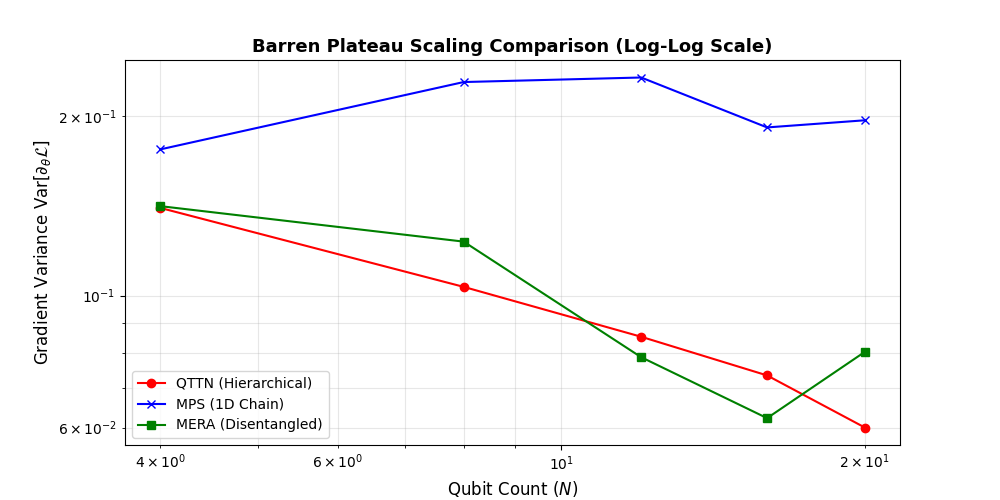
\includegraphics[width=0.8\textwidth]{ch3/topology_barren_plateaus.png}
    \caption{Empirical gradient variance scaling. All three tensor networks exhibit polynomial rather than exponential decay at the tested scales, successfully avoiding a barren plateau.}
    \label{fig:topology_barren_plateaus}
\end{figure}

For the QTTN, this empirical success is theoretically guaranteed. Pesah et al. \cite{pesah2021_qcnn} proved that hierarchical topologies avoid barren plateaus because the gradient depends only on a bounded causal cone scaling logarithmically ($\mathcal{O}(\log N)$). However, this theoretical guarantee does not extend to 1D MPS or standard MERA networks. Their survival in this specific diagnostic is an empirical artifact of the shallow depths and bounded scales ($N \le 20$) tested. Nonetheless, at the operational scales required for our vision task, the gradient variance of all architectures remained highly stable and optimizable.


\subsection{Ansatz and Encoding Investigation}

Having established the baseline trainability of the QTTN topology, the next phase of optimization focused on its internal node mechanics. The representational capacity of a quantum node is dictated by the pairing of its classical-to-quantum encoding strategy and its parameterized ansatz. 

\subsubsection{Documenting the Search Space}
\label{sec:search_space}
To broadly explore the available architectural space, we executed a combinatorial sweep across the four encoding strategies defined in Section \ref{sec:enc_scalar_ry}--\ref{sec:enc_zz_map} (\texttt{scalar\_ry}, \texttt{multi\_axis}, \texttt{amplitude} and \texttt{zz\_map}) and the three ans\"{a}tze of Section \ref{sec:ansatz_design} (HEA, ALT and IQP), giving twelve configurations. The results are shown in Figure \ref{fig:encoding_ansatz_survey}.

Two constraints bound what this diagnostic can establish. First, it was executed on a downsampled $8 \times 8$ dataset using a single 4-qubit quantum node rather than the full hierarchical tree, so it characterises node-level circuits and not the tower. Second, the four-class dataset admits a \textit{single-attribute ceiling} at $50\%$: colour alone separates two of the four classes from the other two, as does shape, so either attribute in isolation caps at $50\%$ and any score materially above it requires binding colour to shape. This makes the ceiling, rather than the $25\%$ chance floor, the meaningful reference line.

\begin{figure}[hbt!]
    \centering
    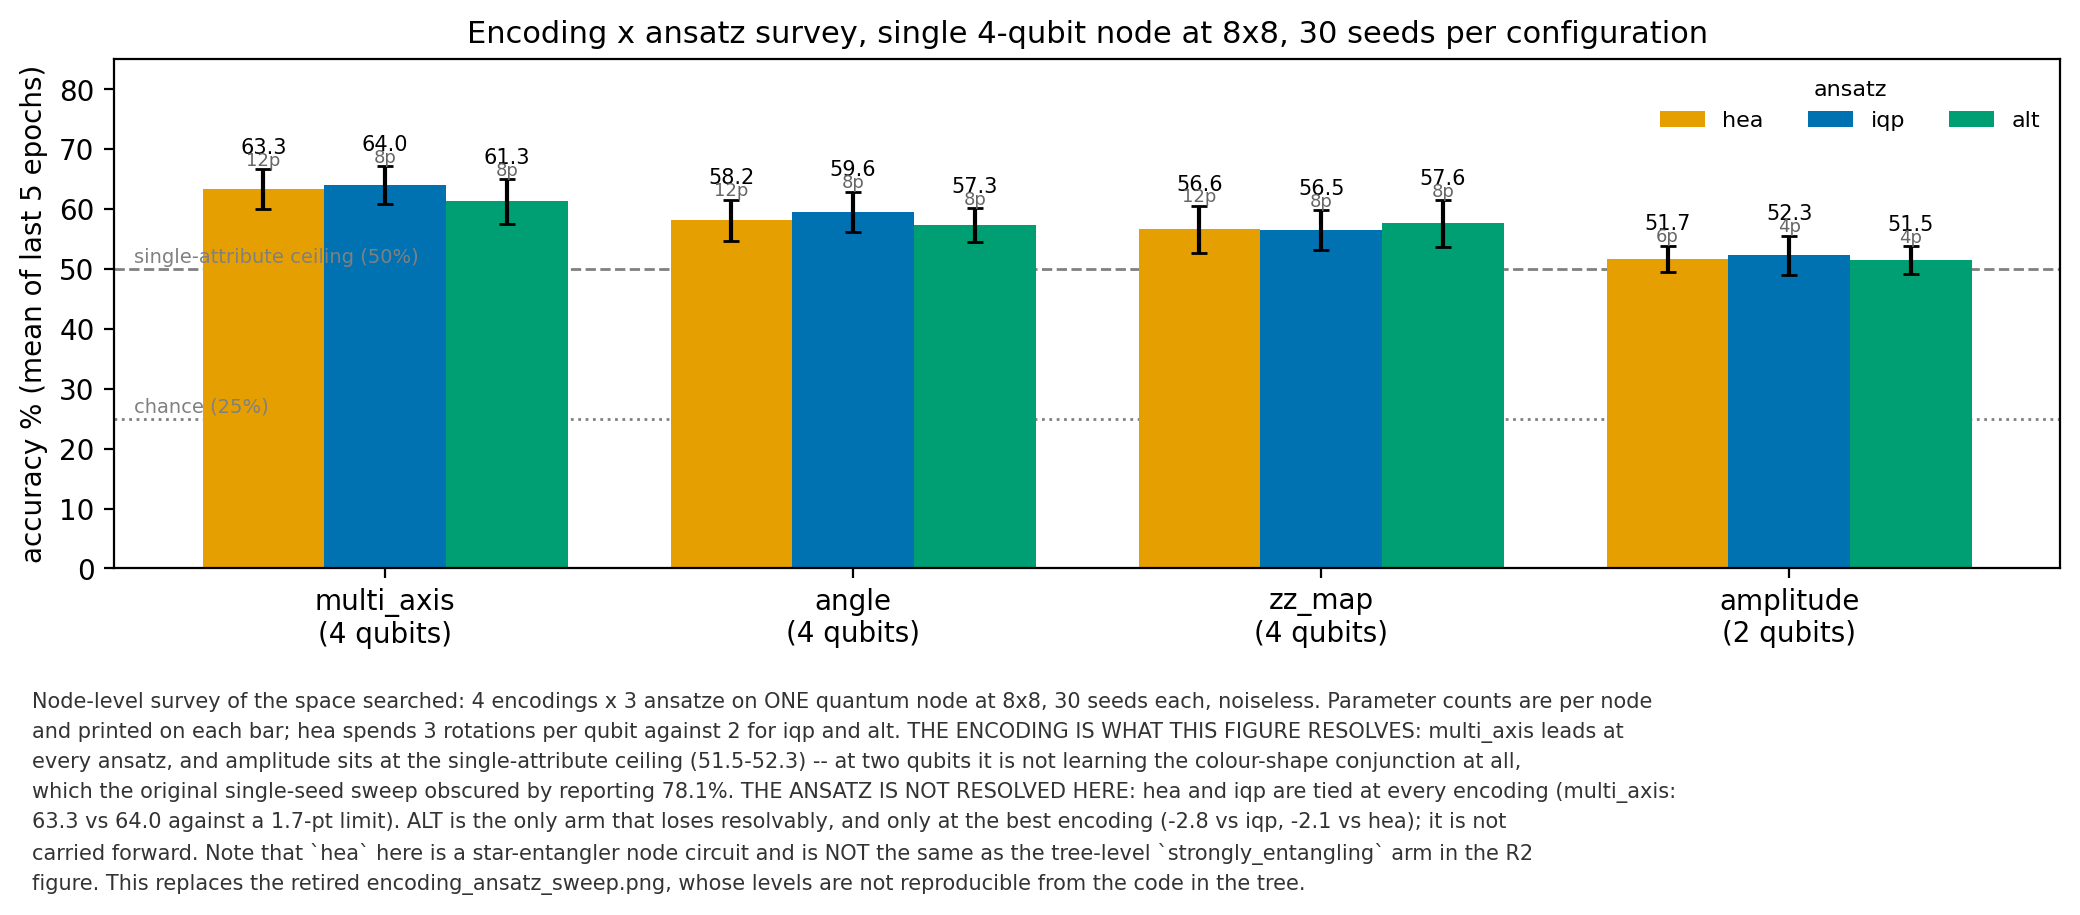
\includegraphics[width=1.0\textwidth]{ch3/encoding_ansatz_survey.png}
    \caption{Node-level survey of the search space: four encodings $\times$ three ans\"{a}tze on a single 4-qubit node at $8 \times 8$, 30 seeds per configuration, noiseless. The \texttt{multi\_axis} encoding leads at every ansatz, while \texttt{amplitude} sits at the $50\%$ single-attribute ceiling.}
    \label{fig:encoding_ansatz_survey}
\end{figure}

Three observations follow. The \texttt{multi\_axis} encoding leads at every ansatz, reaching $64.0\%$ against $59.6\%$ for \texttt{scalar\_ry}, $56.5\%$ for \texttt{zz\_map} and $52.3\%$ for \texttt{amplitude}. The direction of that result is confirmed independently, and at far greater statistical strength, on the full tree in the next section.

The \texttt{amplitude} encoding, by contrast, sits at $51.5$--$52.3\%$ across all three ans\"{a}tze --- that is, exactly at the single-attribute ceiling. Compressing four patches into two qubits is the most qubit-efficient option available, but at this width the encoding does not learn the colour--shape conjunction at all; it resolves one attribute and stops. Qubit economy is therefore not free, and \texttt{amplitude} is eliminated here rather than carried forward.

The ansatz, however, is \textit{not} resolved by this survey. HEA and IQP are statistically tied at every encoding, differing by $0.7$ points at \texttt{multi\_axis} against a resolution limit of $1.7$. ALT is the only arm that loses resolvably, and only at the best encoding ($-2.8$ against IQP and $-2.1$ against HEA, both past their limits); it is not carried forward. The two surviving ans\"{a}tze were therefore taken to a stricter evaluation at the full image resolution, on the full tree.

\subsubsection{Rigorous Hybrid-Tree Evaluation}
\label{sec:hybrid_eval}
To definitively resolve the optimal configuration, the surviving candidates from the survey were subjected to a rigorous evaluation using 21 independent random seeds on the $16 \times 16$ dataset (1024 train / 64 test). At this scale the hardware-efficient arm is PennyLane's standard \texttt{StronglyEntanglingLayers}, denoted \texttt{strongly\_entangling}, in preference to the hand-rolled node circuit used in the survey; the two are members of the same family but are not identical circuits, so the absolute figures are not comparable across the two scales.

Importantly, this ranking was established using a \textit{hybrid} tree architecture (the measure-and-re-encode topology). In this framework, every node builds its own 4-qubit device, and the levels communicate by passing classical scalar measurements, completely bypassing the need for a massive coherent 16-qubit register. Statistical significance across the configurations was determined using Welch's unequal variances t-test to calculate the Minimum Detectable Effect (MDE).

As shown in Figure \ref{fig:encoding_ansatz}, transitioning from the \texttt{scalar\_ry} encoding (113 parameters) to the \texttt{multi\_axis} encoding (211 parameters) yielded a massive $+12.9$ point improvement in mean accuracy on the hybrid tree. Because this difference vastly exceeded the statistical resolution limit ($\text{MDE} = 3.7$), the absolute superiority of the \texttt{multi\_axis} encoding was definitively resolved.

\begin{figure}[hbt!]
    \centering
    
\includegraphics[width=1.0\textwidth]{ch3/encoding_ansatz.png}
    \caption{Encoding and Ansatz configuration sweep on the hybrid tree ($16 \times 16$ images) across 21 seeds. The \texttt{multi\_axis} encoding yields a statistically resolved $+12.9$ point improvement.}
    \label{fig:encoding_ansatz}
\end{figure}

With the encoding established, we evaluated the parameterized ansatz, comparing the \texttt{strongly\_entangling} baseline against the structured \texttt{iqp} ansatz. The result reproduces the survey's verdict at greater strength: the two ans\"{a}tze are statistically tied. The IQP ansatz achieved a mean accuracy of $80.9\%$, edging out the strongly entangling ansatz at $79.3\%$, but as shown in Figure \ref{fig:ansatz_comparison} this $+1.6$ point difference falls strictly below the statistical resolution limit ($\text{MDE} = 4.8$). The ansatz is therefore unresolved on accuracy at both scales, and the choice must be made on other grounds.

\begin{figure}[hbt!]
    \centering
    
\includegraphics[width=1.0\textwidth]{ch3/ansatz_comparison.png}
    \caption{Per-seed spread for the \texttt{strongly\_entangling} vs. \texttt{iqp} ans\"{a}tze on the hybrid tree. The difference in mean accuracy is statistically unresolved.}
    \label{fig:ansatz_comparison}
\end{figure}

Despite the statistical tie in raw accuracy, the \texttt{iqp} ansatz was selected for two structural reasons. First, it demonstrated a tighter spread across the 21 seeds (standard deviation of $4.9$ vs $9.7$), indicating more stable training, which buys resolution on every comparison downstream. Second, the IQP circuit enforces a rigid inductive bias using commuting, diagonal operations, which requires a shallower physical gate depth. Since the accuracy comparison is a tie at both the node and the tree scale, these are the operative criteria; the two arms are allocated identical parameter budgets here, so parameter economy does not discriminate between them.\footnote{The two ans\"{a}tze share a $[\,\text{layers} \times \text{qubits} \times 3\,]$ weight tensor so that the arms are exactly parameter-matched, of which IQP uses two of the three rotation columns. At the single-node scale of the survey, where the circuits were implemented independently, IQP is genuinely the cheaper of the two (8 parameters against 12).}

This winning node configuration—the highly expressive \texttt{multi\_axis} encoding paired with the stable, shallow \texttt{iqp} ansatz—was subsequently adopted and ported directly into the fully coherent 16-qubit QTTN (evaluated later in this chapter) as the architecture of record.

\subsection{Solving the Readout Bottleneck}
% - Detail the critical discovery: The single marginal readout bottlenecked the model's bandwidth.
% - State the finding: Transitioning to the 4-wire multi-Pauli readout closed a massive 43-point accuracy gap.
% - FIGURES: Reference readout_bottleneck.png.

Following the resolution of the internal node mechanics, we evaluated the final component of the architecture: the classical readout protocol. As theorized in Section \ref{sec:readout_protocols}, the hierarchical tensor topology aggressively traces out leaf qubits at each layer, forcing all spatial reasoning to funnel into the final root node.

In an ideal, unconstrained physical quantum computer, this severe information funnel would be resolved by simply increasing the bond dimension between nodes (i.e., passing multiple qubits from the leaf layers up to the root, exponentially increasing $\chi$). Given a sufficiently large bond dimension, taking the expectation value of a single marginal qubit at the root would theoretically provide enough bandwidth for the classical loss function to train the network.

However, as established by the simulation constraints in Chapter \ref{ch:theory}, our investigation is strictly bounded to a 16-qubit architecture by the classical limits of statevector simulation. In a quantum tensor network, the bond dimension $\chi$ is defined by the number of qubits $n$ passed between adjacent nodes ($\chi = 2^n$). Because of our 16-qubit limit, we can only afford to pass $1$ qubit from each child block up to the parent layer. This imposes a hard, physical limit on the internal bond dimension of exactly $\chi = 2$. 
When evaluating the model using the standard single marginal readout ($\langle Z_0 \rangle$) under this severely constrained bond dimension, the network suffered from a catastrophic information bottleneck, capping its classification accuracy.

To circumvent this simulation limitation without adding auxiliary qubits (which would trigger the density matrix memory wall), we transitioned from a single marginal readout to a multi-wire observable strategy on the surviving top-layer qubits. Instead of measuring a single root wire, this protocol measures observables across all four surviving parent qubits before the final contraction (e.g., measuring $\langle Z_0 \rangle, \langle Z_1 \rangle, \langle Z_2 \rangle, \langle Z_3 \rangle$ and feeding them into a classical dense layer).

As illustrated in Figure \ref{fig:readout_bottleneck}, this architectural adjustment artificially widened the effective bond dimension at the top of the tree, allowing the model to project a richer, multi-dimensional representation of the tree's final state to the classical optimizer. Empirically, this multi-wire workaround was transformational, closing a massive 43-point accuracy gap. 

It is important to state explicitly that while this multi-readout protocol is strictly necessary for our constrained 16-qubit simulation, it is fully expected that a physical quantum device running a TTN with a larger internal bond dimension would achieve comparable results using a standard, hardware-efficient single marginal readout.

\begin{figure}[hbt!]
    \centering
    % Insert the readout bottleneck / multi-pauli comparison figure here
    
\includegraphics[width=0.8\textwidth]{ch3/readout_bottleneck.png}
    \caption{Empirical validation of the readout bottleneck. Transitioning from a single marginal readout ($\langle Z \rangle$) to a multi-wire readout on the top layer artificially widens the restricted bond dimension, closing a 43-point accuracy gap caused by simulation limits.}
    \label{fig:readout_bottleneck}
\end{figure}

\subsection{Dropout and Residuals: Porting Classical Mechanisms}
\label{sec:ablations}
% - Detail the noise sweeps: Present the empirical effect of simulated quantum noise (e.g., depolarizing channels) on the surviving ansätze. Which ansatz was most resilient?
% - Detail the ablation tests: Classical residuals and spatial ancilla qubits failed to justify their parameter cost or triggered the Density Matrix Wall, leading to their rejection.
% - FIGURES: Reference ablations_and_noise.png.

With the baseline node architecture resolved, we conducted a final series of evaluations to determine if we could port highly successful mechanisms from classical Deep Learning directly into the quantum tensor network. Specifically, we investigated quantum analogs for Dropout regularization, Residual skip connections, and explicit positional embeddings.
We evaluated the following node-level modifications:
\begin{enumerate}
    \item \textbf{Quantum Dropout via Depolarizing Noise:} In classical networks, Dropout \cite{srivastava2014dropout} prevents overfitting by randomly nullifying activations. We subjected our architectures to varying depolarizing noise channels ($p$) to determine if quantum noise could act as a structural equivalent to Dropout, thereby serving as an effective regularizer.
    \item \textbf{Classical Residuals (\texttt{mixed\_channel}):} Inspired by classical ResNets \cite{he2016resnet}, this mechanism attempts to port residual skip connections into the quantum domain by allowing certain classical feature channels to bypass the quantum node entirely, preserving classical gradients.
    \item \textbf{Spatial Ancillae (\texttt{with\_ancilla}):} Allocating an auxiliary qubit to explicitly encode spatial positional embeddings, mimicking the positional tokens used in classical Vision Transformers (ViTs) \cite{dosovitskiy2020vit}.
    \item \textbf{Data Re-uploading (\texttt{reupload}):} Re-injecting classical features deep into the ansatz to artificially increase non-linearity, following the protocol established by Pérez-Salinas et al. \cite{perez_salinas_2020}.
\end{enumerate}
These ablations were executed on the hybrid tree across 30 random seeds. Crucially, as theorized in Chapter \ref{ch:theory}, simulating quantum noise requires density matrix emulation, the memory footprint of which scales exponentially at $\mathcal{O}(4^N)$. Because full-tree emulation is computationally intractable under the Density Matrix Wall, the noise characterization was strictly bounded to the single-node scale.
The empirical results, shown in Figure \ref{fig:ablations_and_noise}, decisively rejected the translation of these classical mechanisms into the quantum architecture. 
\begin{figure}[hbt!]
    \centering
    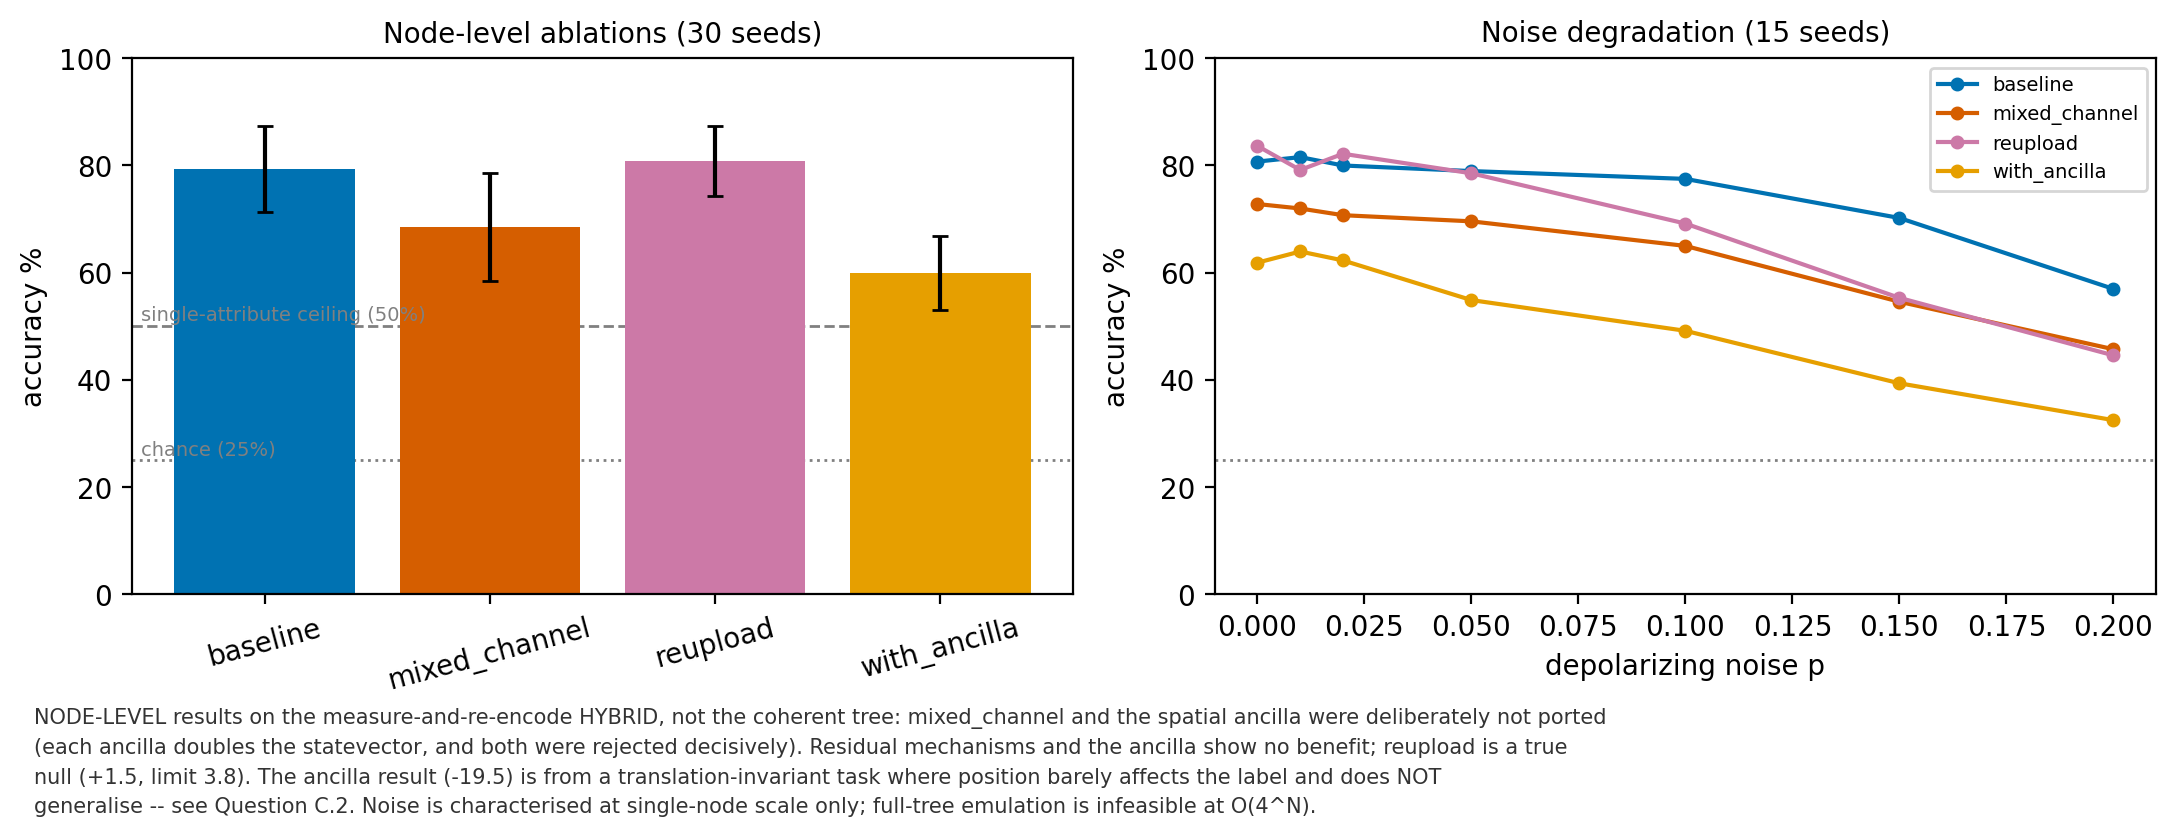
\includegraphics[width=1.0\textwidth]{ch3/ablations_and_noise.png}
    \caption{Node-level ablations (30 seeds) and noise degradation sweeps (15 seeds). The attempts to port classical mechanisms yielded either true null results (\texttt{reupload}) or actively harmed performance (\texttt{mixed\_channel}, \texttt{with\_ancilla}) while degrading noise resilience.}
    \label{fig:ablations_and_noise}
\end{figure}
The \texttt{reupload} mechanism achieved a nominal $+1.5$ point increase over the baseline; however, this fell well below the statistical resolution limit ($\text{MDE} = 3.8$), yielding a true statistical null that failed to justify its additional gate depth. 
The \texttt{mixed\_channel} approach—our attempt to port ResNet skip connections—actively harmed performance, dragging mean accuracy down significantly. Most severely, the \texttt{with\_ancilla} positional embedding triggered a catastrophic $-19.5$ point drop in accuracy. Because the Synthetic Shapes dataset evaluates a largely translation-invariant classification task, explicitly encoding positional data into a spatial ancilla provided no predictive benefit. Conversely, because each ancilla qubit doubles the required statevector dimension, it drastically increased the computational burden for zero gain.
Finally, the noise degradation sweep revealed that the simple \texttt{baseline} architecture was notably more resilient to depolarizing channels than any of the complex alternatives, and that noise strictly degraded performance rather than acting as a beneficial "Quantum Dropout" regularizer. Consequently, classical residuals and spatial ancillae were deliberately discarded. The lean, baseline node architecture proved to be the mathematically optimal balance of accuracy, hardware efficiency, and noise resilience.

\section{Model Parameter Efficiency}

This section pits the fully optimized quantum tensor network against classical tensor and neural benchmarks to probe parameter efficiency. The winning node configuration---the \texttt{multi\_axis} encoding paired with the \texttt{iqp} ansatz and the multi-Pauli readout---was ported into a fully coherent 16-qubit QTTN and compared against five baselines:

\begin{enumerate}
    \item \textbf{\texttt{mlp\_reference}:} A standard, unstructured Multi-Layer Perceptron, deliberately over-provisioned to establish the accuracy ceiling of the dataset.
    \item \textbf{\texttt{mlp\_param\_matched}:} The same architecture shrunk to approximately the quantum model's parameter budget, which separates the effect of structure from the effect of capacity.
    \item \textbf{\texttt{classical\_bare}:} A classical tensor network using Canonical Polyadic (CP) decomposition with a swept rank --- the direct structural analogue to the quantum tree under matched constraints, with no residual connections and no dropout.
    \item \textbf{\texttt{classical\_full}:} The same CP tree equipped with the residual connections and dropout that the quantum node was shown in Section \ref{sec:ablations} not to benefit from.
    \item \textbf{\texttt{quantum\_hybrid}:} The measure-and-re-encode tree of Section \ref{sec:hybrid_eval}, retained here to quantify what passing intermediate states as qubits rather than as classical scalars is worth.
\end{enumerate}

\begin{table}[hbt!]
    \centering
    \begin{tabular}{l c c}
        \toprule
        \textbf{Architecture} & \textbf{Parameters} & \textbf{Accuracy} \\
        \midrule
        \texttt{mlp\_reference}    & 999 & $96.0 \pm 1.5$ \\
        \midrule
        \textbf{\texttt{quantum\_coherent}} & \textbf{287} & $\mathbf{89.3 \pm 3.9}$ \\
        \texttt{classical\_full} (CP + residual + dropout) & 352 & $88.4 \pm 5.5$ \\
        \texttt{classical\_bare} (CP) & 428 & $79.6 \pm 10.3$ \\
        \texttt{quantum\_hybrid} & 211 & $79.4 \pm 8.0$ \\
        \texttt{mlp\_param\_matched} & 257 & $70.5 \pm 18.1$ \\
        \bottomrule
    \end{tabular}
    \caption{Parameter efficiency on $16 \times 16$ synthetic shapes (1024 train / 64 test, scored on the mean of the last five epochs). The coherent quantum tree is the second most accurate model in the comparison at less than a third of the parameters of the model above it.}
    \label{tab:model_comparison}
\end{table}

The results are given in Table \ref{tab:model_comparison} and Figure \ref{fig:model_comparison}. Three of the four comparisons resolve against the Welch limit, and the fourth is a tie that matters.

\begin{figure}[hbt!]
    \centering
    
\includegraphics[width=1.0\textwidth]{ch3/model_comparison.png}
    \caption{Final parameter efficiency comparison. The 287-parameter coherent QTTN outperforms the structurally equivalent classical tensor network despite a strict parameter deficit, and ties the augmented classical tree that carries residual connections and dropout.}
    \label{fig:model_comparison}
\end{figure}

Against \texttt{classical\_bare}, its direct structural analogue, the quantum model gains $+9.7$ points (limit $6.3$) while using $33\%$ fewer parameters. This is the central result of the chapter: under matched constraints the unitary restriction does not cost representational capacity, and on this task it appears to act as a structural regularizer rather than a handicap.

Against \texttt{classical\_full} the two are \textit{tied} ($89.3$ against $88.4$). This is worth stating explicitly rather than presenting the \texttt{classical\_bare} comparison alone, because it is the stronger claim of the two: the quantum tree matches the best classical tensor network in the study while using $19\%$ fewer parameters \textit{and} without the residual connections and dropout that the classical arm depends on --- mechanisms which, as Section \ref{sec:ablations} showed, actively harm the quantum node when ported to it. The classical tree needs them; the quantum tree reaches the same accuracy without them.

Against \texttt{quantum\_hybrid} the coherent tree gains $+9.9$ points (limit $5.7$), which is what justifies the coherent topology over the simpler measure-and-re-encode design. Against \texttt{mlp\_param\_matched} it gains $+18.8$ points (limit $9.0$), establishing that at this parameter budget the hierarchical contraction is doing work that an unstructured network of the same size cannot.

Two qualifications belong with these numbers. First, the 999-parameter \texttt{mlp\_reference} leads the entire comparison at $96.0\%$; the claim here concerns the quantum node against its \textit{structural} counterparts at matched capacity, not against classical vision at unrestricted capacity. Second, the classical arms were hyperparameter-tuned while the quantum arm inherited its learning rate from an earlier task, so the comparison is conservative in the quantum model's favour.


\section{Architectural Verdict}
% Explicitly declare the winner: The 287-parameter QTTN (with IQP, multi-axis encoding, and multi-Pauli readout) alongside the tuned classical controls will advance to the CLEVR compositional benchmarks in Chapter 5.

Following the exhaustive empirical diagnostics conducted across this chapter, the optimal architectural configuration of the model has been definitively resolved. 
The fully coherent, 287-parameter Quantum Tree Tensor Network (QTTN)—constructed utilizing the \texttt{multi\_axis} encoding strategy, the parameter-efficient \texttt{iqp} ansatz, and a multi-Pauli top-layer readout—has mathematically proven its trainability, stability, and extreme parameter efficiency on synthetic spatial reasoning tasks. 
Having successfully established this robust perception baseline, this specific quantum architecture, alongside its classical tensor controls (\texttt{classical\_bare} and \texttt{classical\_full}), will advance to the next phase of the investigation. Definitions for all three models are given in Appendix \ref{appendix:models}.


% ==========================================
% CHAPTER 5: CLEVR
% ==========================================

\chapter{CLEVR: Relational and Compositional Evaluation}
\label{ch:clevr}
% TODO: regenerate the figures with better captions

Having established a robust quantum perception baseline on synthetic shapes, this chapter transitions the investigation to the CLEVR dataset \cite{johnson2017clevr}. CLEVR serves as a definitive diagnostic benchmark for visual reasoning, providing complex 3D scenes populated with multiple interacting objects. Each object exhibits distinct visual attributes (colour, shape, material, size) and rigorous spatial positioning. By deploying our surviving Quantum Tree Tensor Network (QTTN) and classical tensor controls on this dataset, we aim to answer the core structural question of this thesis: whether quantum tensor topologies can naturally encode spatial geometry and resolve compositional binding better than unconstrained classical alternatives.

\section{Methodology and Aims}
To rigorously map the architectural limits of tensor networks, our evaluation on the CLEVR dataset is structured across an escalating hierarchy of visual reasoning. We define a three-stage progression:
\begin{enumerate}
    \item \textbf{Perception:} Scaling the models to extract the full 15-class attribute space to establish a baseline of visual competency in multi-object scenes.
    \item \textbf{Spatial Relations:} Evaluating the implicit geometric hierarchy of the quad-tree on explicit spatial routing tasks.
    \item \textbf{Compositional Binding:} Confronting the models with the binding problem \cite{greff2020binding} to test if they can structurally associate features with distinct spatial entities.
\end{enumerate}

The remainder of this section details the dataset adaptations and task definitions required to execute this progression.

\subsection{Dataset Adaptation: World-Scaled Cropping}
Before the models could evaluate CLEVR scenes, the data had to be processed into object crops suitable for our 16-qubit input boundary, that is, a $4 \times 4$ grid of patches. However, naive 2D bounding-box cropping introduces a geometric confound: a physically "large" object and a "small" object will both be rescaled to fill $100\%$ of the crop window, rendering the model entirely blind to the \texttt{size} attribute. Furthermore, perspective projection means a small object close to the camera can appear identical to a large object far away.

To resolve this, we engineered a depth-invariant, world-scaled cropping methodology governed by a global calibration constant, \texttt{CROP\_K}. The pixel width of the crop is calculated strictly as a function of the object's 3D distance from the camera:
\begin{equation}
    \text{Crop Side (px)} = \frac{\texttt{CROP\_K}}{\text{Depth}}
\end{equation}

By scaling the crop window inversely with depth, the crop captures a constant physical area of the 3D world. Within this fixed window, the proportion of the image filled by the object becomes a direct, depth-invariant measure of its true physical radius.

\begin{figure}[hbt!]
    \centering
    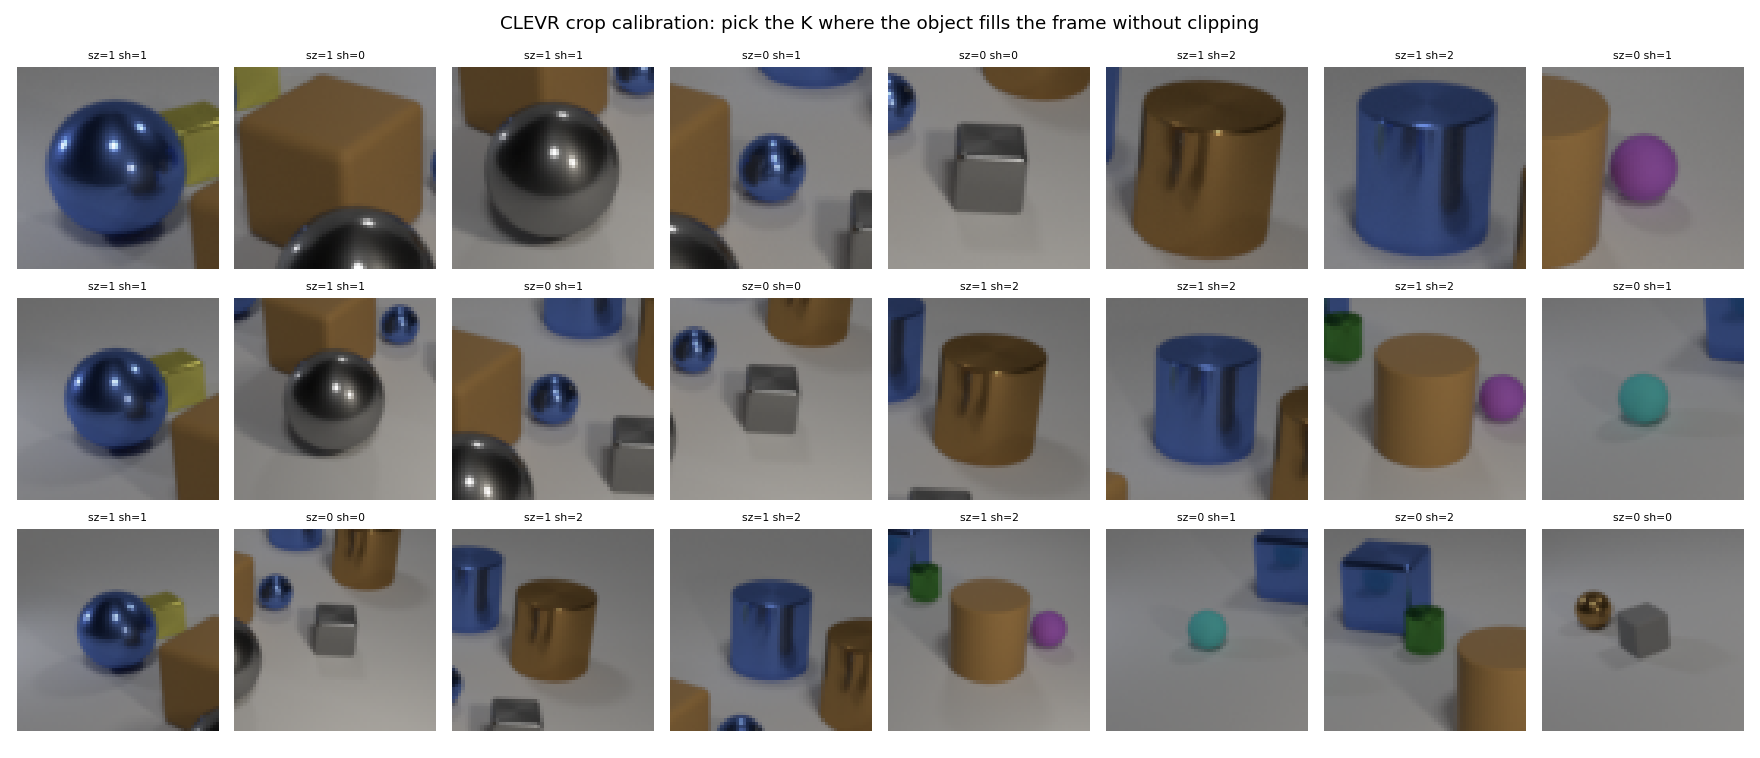
\includegraphics[width=0.8\textwidth]{ch3/clevr_crop_calibration.png}
    \caption{World-scaled cropping calibration (\texttt{CROP\_K} = 1470.0). By anchoring the crop size to 3D depth rather than 2D pixel bounds, physically large objects (right) consistently fill a larger fraction of the crop window than small objects (left), preserving the \texttt{size} attribute.}
    \label{fig:clevr_crop}
\end{figure}

As shown in Figure \ref{fig:clevr_crop}, this adaptation mathematically isolates the true physical dimensions of the object, ensuring the \texttt{size} attribute remains highly learnable alongside colour, shape, and material.

\subsection{Defining the Relational Task}
To evaluate the second stage of our progression, we derived explicit relational tasks from the CLEVR scenes (Left, Right, Front, Behind), as shown in Figure \ref{fig:clevr_relations}.

\begin{figure}[hbt!]
    \centering
    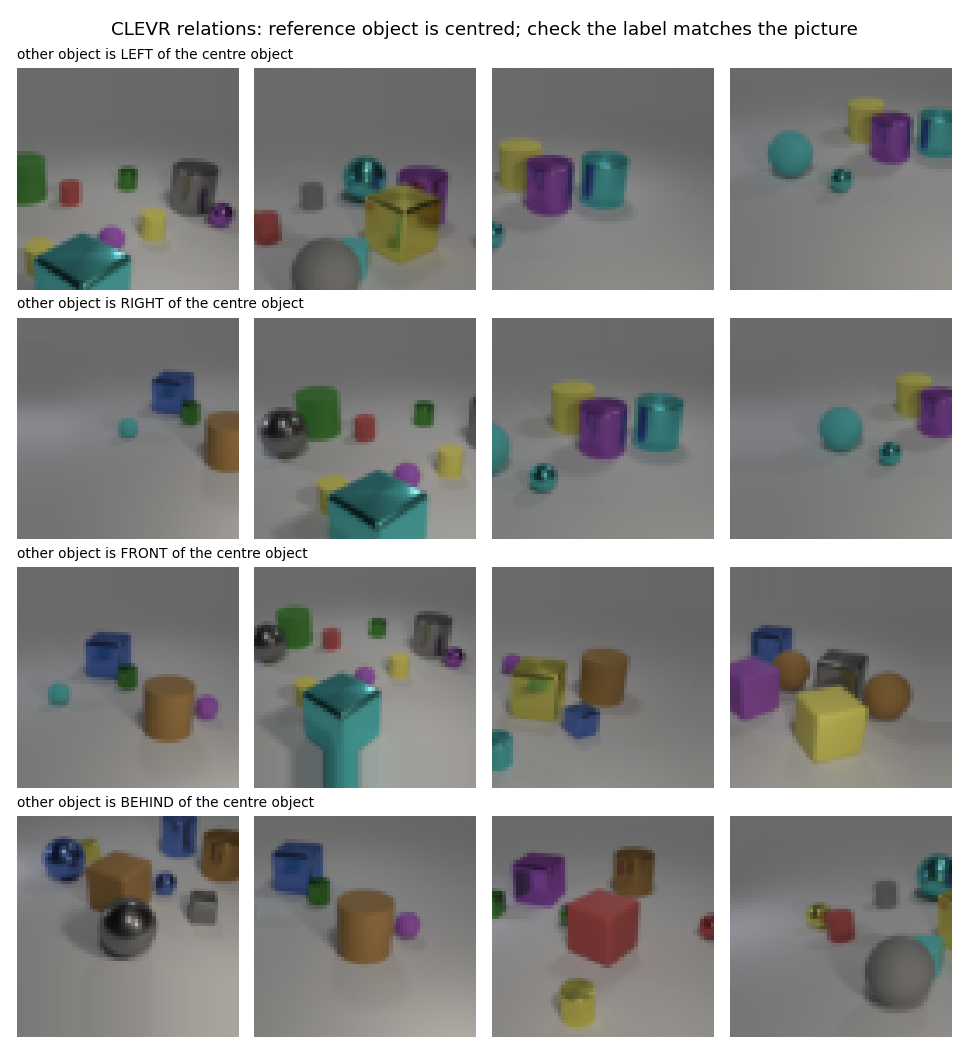
\includegraphics[width=0.9\textwidth]{ch3/clevr_relation_examples.png}
    \caption{Spatial relation tasks derived from CLEVR, requiring the model to resolve explicit geometric relationships between distinct compositional entities.}
    \label{fig:clevr_relations}
\end{figure}

This task serves as a direct diagnostic of whether the implicit geometric hierarchy of the tensor network—specifically, the way image patches are structurally routed through the tree—naturally encodes spatial geometry, or if explicit positional embeddings are required for spatial awareness.

\subsection{Defining the Compositional Binding Probe}
The final and most rigorous stage of the progression targets the binding problem. While human perception inherently binds visual features to specific physical entities, standard neural networks often confuse which attributes belong to which object when observing complex scenes.

To evaluate this, we define a rigorous Compositional Binding Probe. The models are tasked with distinguishing between scenes that contain the exact same raw features, but in swapped configurations (e.g., distinguishing a [red square, blue circle] from a [blue square, red circle]), as seen in Figure \ref{fig:clevr_binding}. Because each probe image is a composite of two objects rather than a single crop, this stage is run at $32 \times 32$ rather than the $16 \times 16$ used elsewhere in this chapter. The circuit is unchanged at 16 qubits; only the patches, and hence the classical embedding layer feeding them, are larger, which is why every arm carries more parameters here.

\begin{figure}[hbt!]
    \centering
    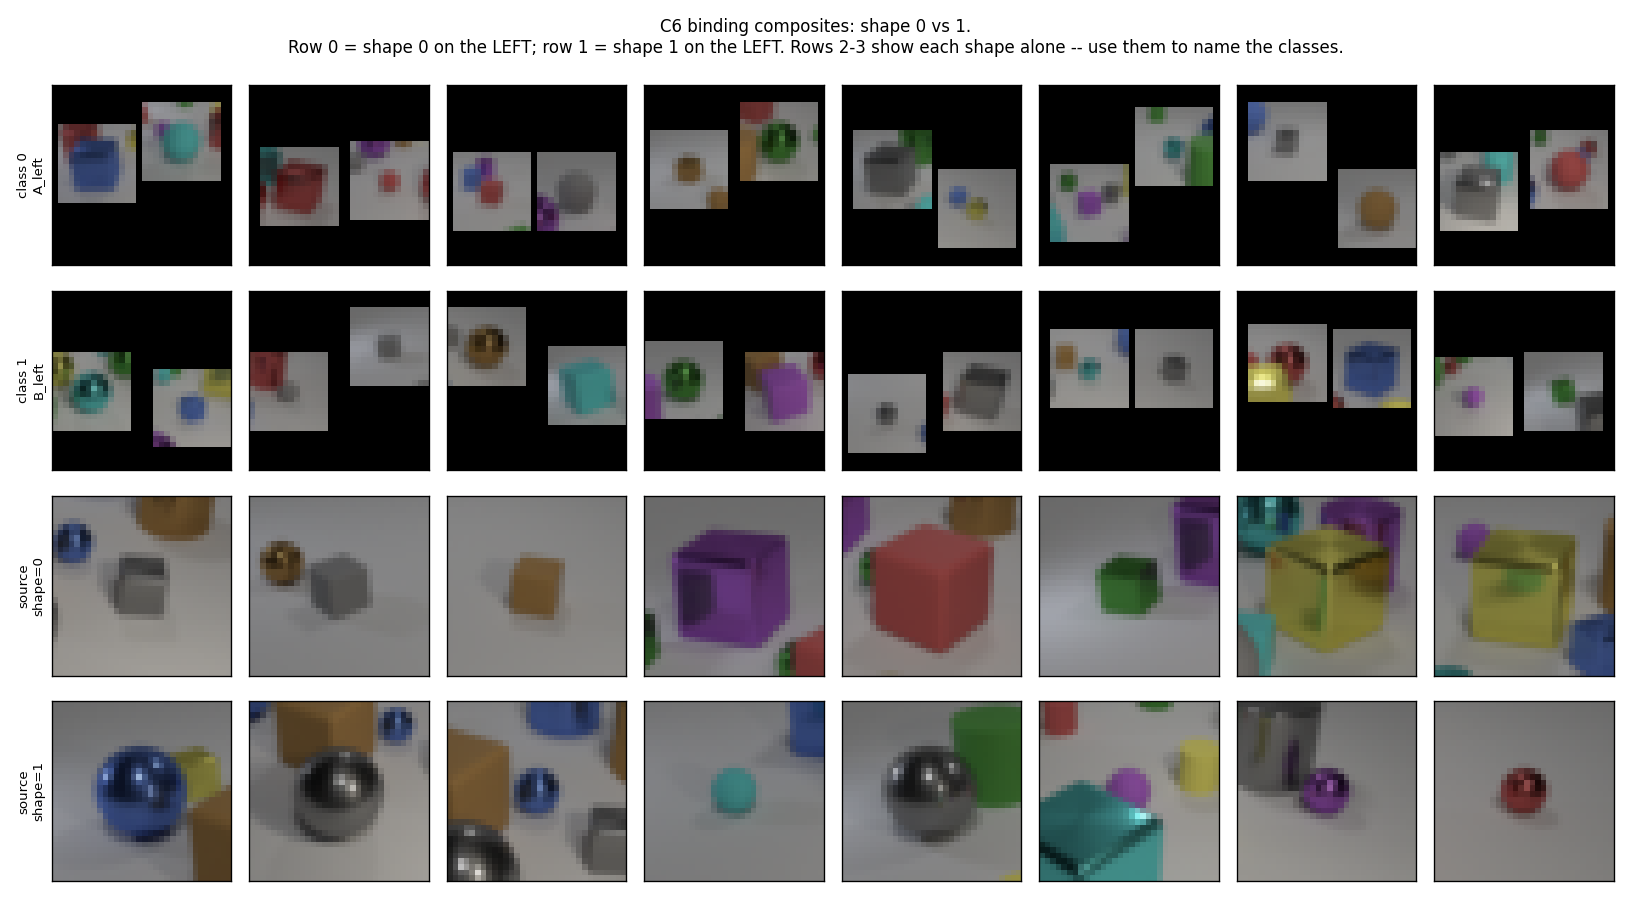
\includegraphics[width=0.9\textwidth]{ch3/clevr_binding_examples.png}
    \caption{Examples from the CLEVR Compositional Binding Probe. The model must learn to bind attributes to specific spatial entities to distinguish between configuration swaps.}
    \label{fig:clevr_binding}
\end{figure}

If an architecture simply acts as a "bag of features" without the structural capacity to bind those features to distinct spatial locations, it will fail to separate these swapped configurations.

\section{Perception and the Multi-Head Architecture}
% - Scaling the head for 15 classes (colour, shape, material, size), pushing the quantum model to 462 parameters.
% - Perception results: the quantum tower beats the 551-parameter classical_full on shape and material at 30 epochs.

To execute the first stage of our evaluation progression, we established a perception baseline on the processed CLEVR images. Unlike the synthetic dataset in Chapter \ref{ch:synthetic} (which evaluated a single 4-class shape target), the CLEVR dataset requires the simultaneous classification of 15 distinct attribute classes across four independent dimensions: 8 colours, 3 shapes, 2 materials, and 2 sizes.

To achieve this, the model was upgraded to a multi-head architecture. Instead of a single linear layer, four independent linear heads—one for each attribute dimension—were attached to the final top-layer multi-Pauli measurement of the tree. Crucially, all four heads draw from the exact same underlying quantum measurement vector. Consequently, the quantum network is forced to learn a rich, highly entangled representation capable of resolving all 15 classes simultaneously within its strict qubit constraints. 

Accommodating these additional classification heads increased the parameter footprint of the fully coherent Quantum Tree Tensor Network (QTTN) to 462 parameters. To ensure a capacity-matched comparison, the structurally faithful classical tensor control (\texttt{classical\_bare}) was tuned to 563 parameters, while the optimized \texttt{classical\_full} baseline (equipped with residual connections and dropout regularization) scaled to 551 parameters. An unstructured, 1186-parameter classical Multi-Layer Perceptron (\texttt{mlp\_reference}) was also included to establish the dataset's overall task difficulty ceiling.

\begin{figure}[hbt!]
    \centering
    
\includegraphics[width=0.9\textwidth]{ch3/clevr_attributes.png}
    \caption{Attribute extraction performance. The multi-head readout forces the quantum architecture to simultaneously resolve all 15 classes from a single underlying statevector.}
    \label{fig:clevr_attributes}
\end{figure}

The empirical results of this perception evaluation are detailed in Table \ref{tab:perception_results}. Initial diagnostics revealed that while the unstructured MLP networks converged rapidly (reaching 98\% of their final score by epoch 12), the tensor networks required an extended 90-epoch budget specifically to converge the 8-class \texttt{colour} head. The 30-epoch budget used in Chapter \ref{ch:synthetic} was inherited from a four-class task and is simply too short here, so every CLEVR figure reported in this chapter uses the 90-epoch budget. It is worth noting that this is the conservative choice for the argument that follows: at 30 epochs the quantum tower wins on \textit{two} attributes rather than one.

\begin{table}[hbt!]
    \centering
    \begin{tabular}{l c | c c c c}
        \toprule
        \textbf{Architecture} & \textbf{Parameters} & \textbf{Colour} & \textbf{Shape} & \textbf{Material} & \textbf{Size} \\
        \midrule
        \texttt{quantum\_coherent} & \textbf{462} & 63.0\% & \textbf{52.7\%} & 61.0\% & 94.1\% \\
        \midrule
        \texttt{classical\_bare} & 563 & 73.4\% & 43.0\% & 56.5\% & 91.8\% \\
        \texttt{classical\_full} & 551 & 75.8\% & 52.2\% & 65.0\% & 97.7\% \\
        \midrule
        \texttt{mlp\_reference} & 1186 & 93.1\% & 74.1\% & 84.0\% & 98.6\% \\
        \bottomrule
    \end{tabular}
    \caption{CLEVR Perception Baseline (90 Epochs). The 462-parameter quantum model is the smallest tensor network evaluated, yet it achieves a statistically resolved $+9.7$ point win on the \texttt{shape} attribute against the larger 563-parameter \texttt{classical\_bare} control. Performance on material, size, and colour is statistically tied given the variance.}
    \label{tab:perception_results}
\end{table}

This extended training exposed a structural dynamic inherent to multi-head networks: because all four heads share a single summed loss and the heads converge at very different rates, the model must "trade heads" to reach equilibrium. Training long enough for \texttt{colour} over-trains everything else, and the degradation on \texttt{material} and \texttt{size} is resolved rather than incidental. No single budget is therefore optimal for all four heads simultaneously --- a limitation of the protocol rather than of either architecture, and one that applies equally to the classical arms.

However, even at this equilibrium, the unitary-constrained tensor structure demonstrated remarkable parameter efficiency. The 462-parameter quantum model is the smallest tensor network in the comparison, operating at an 18\% parameter deficit to its structurally equivalent \texttt{classical\_bare} baseline (563 parameters). Despite this deficit, it achieved a statistically resolved $+9.7$ point win on the \texttt{shape} attribute (limit $8.6$). On the remaining three attributes (material, size, and colour), the quantum model achieved statistical parity, with gaps falling below the resolution limit imposed by seed variance.

Furthermore, the quantum model matched the shape extraction performance of the optimized 551-parameter \texttt{classical\_full} baseline. Having successfully cleared this rigorous multi-dimensional perception baseline and proven its capacity to extract visual features at state-of-the-art parameter efficiency, the quantum model was qualified to advance to the explicit spatial reasoning tasks.

\section{Spatial Relations}
% - The Left/Right/Front/Behind task.
% - Did the implicit tree topology successfully learn spatial relations?

To evaluate the second stage of our progression, the models were tasked with a four-way spatial relation classification (Left, Right, Front, Behind) on two-object CLEVR crops. Because CLEVR defines these spatial relations against a camera-rotated basis (approximately $49^\circ$ offset from raw world axes), this task tests the network's ability to learn complex geometric transformations rather than simple axis heuristics. The theoretical floor for this classification is a 26.6\% majority-class baseline. Before evaluating the quantum architectures, classical controls successfully established the viability of the task: an unstructured \texttt{mlp\_reference} achieved 65.4\%, and the 428-parameter \texttt{classical\_bare} tensor network 49.6\%. 

While quantum training frequently collapsed to the chance floor, on the runs that successfully converged, the 462-parameter \texttt{quantum\_none} and 494-parameter \texttt{quantum\_on\_wire} models reached 46.2\% and 48.0\% respectively, both statistically tied with the \texttt{classical\_bare} control. Because the performance gaps ($-3.4$ and $-1.6$ points) fall strictly below the minimum detectable effects ($5.3$ and $5.2$), we confirm parity between the unitary quantum node and the classical CP node. These quantum arms ran at the 30-epoch budget rather than the 90 used for perception, and several converged runs were still improving when training stopped, so they are a floor on the architecture's capability rather than a ceiling; the parity result is correspondingly conservative. The critical finding here is that \texttt{quantum\_none} carries absolutely no explicit positional parameters; spatial position enters the network strictly through the fixed assignment of image patches to quantum wires. Achieving parity therefore proves that the implicit geometric hierarchy of the tree topology inherently encodes spatial position. This definitively discharges the earlier failure of the spatial ancilla observed in Chapter \ref{ch:synthetic}, which was measured on a translation-invariant task and provided no signal regarding actual relational reasoning. Whether injecting explicit positional embeddings on top of this implicit structure provides further benefit remains statistically unresolved ($+1.8$ points against a $5.4$ limit), particularly because the \texttt{on\_wire} mechanism introduces an additional 32 parameters, confounding any potential advantage with raw parameter capacity. Ultimately, these results demonstrate that the binding constraint of the quantum architecture is optimization stability, not representational capacity.

\begin{figure}[hbt!]
    \centering
    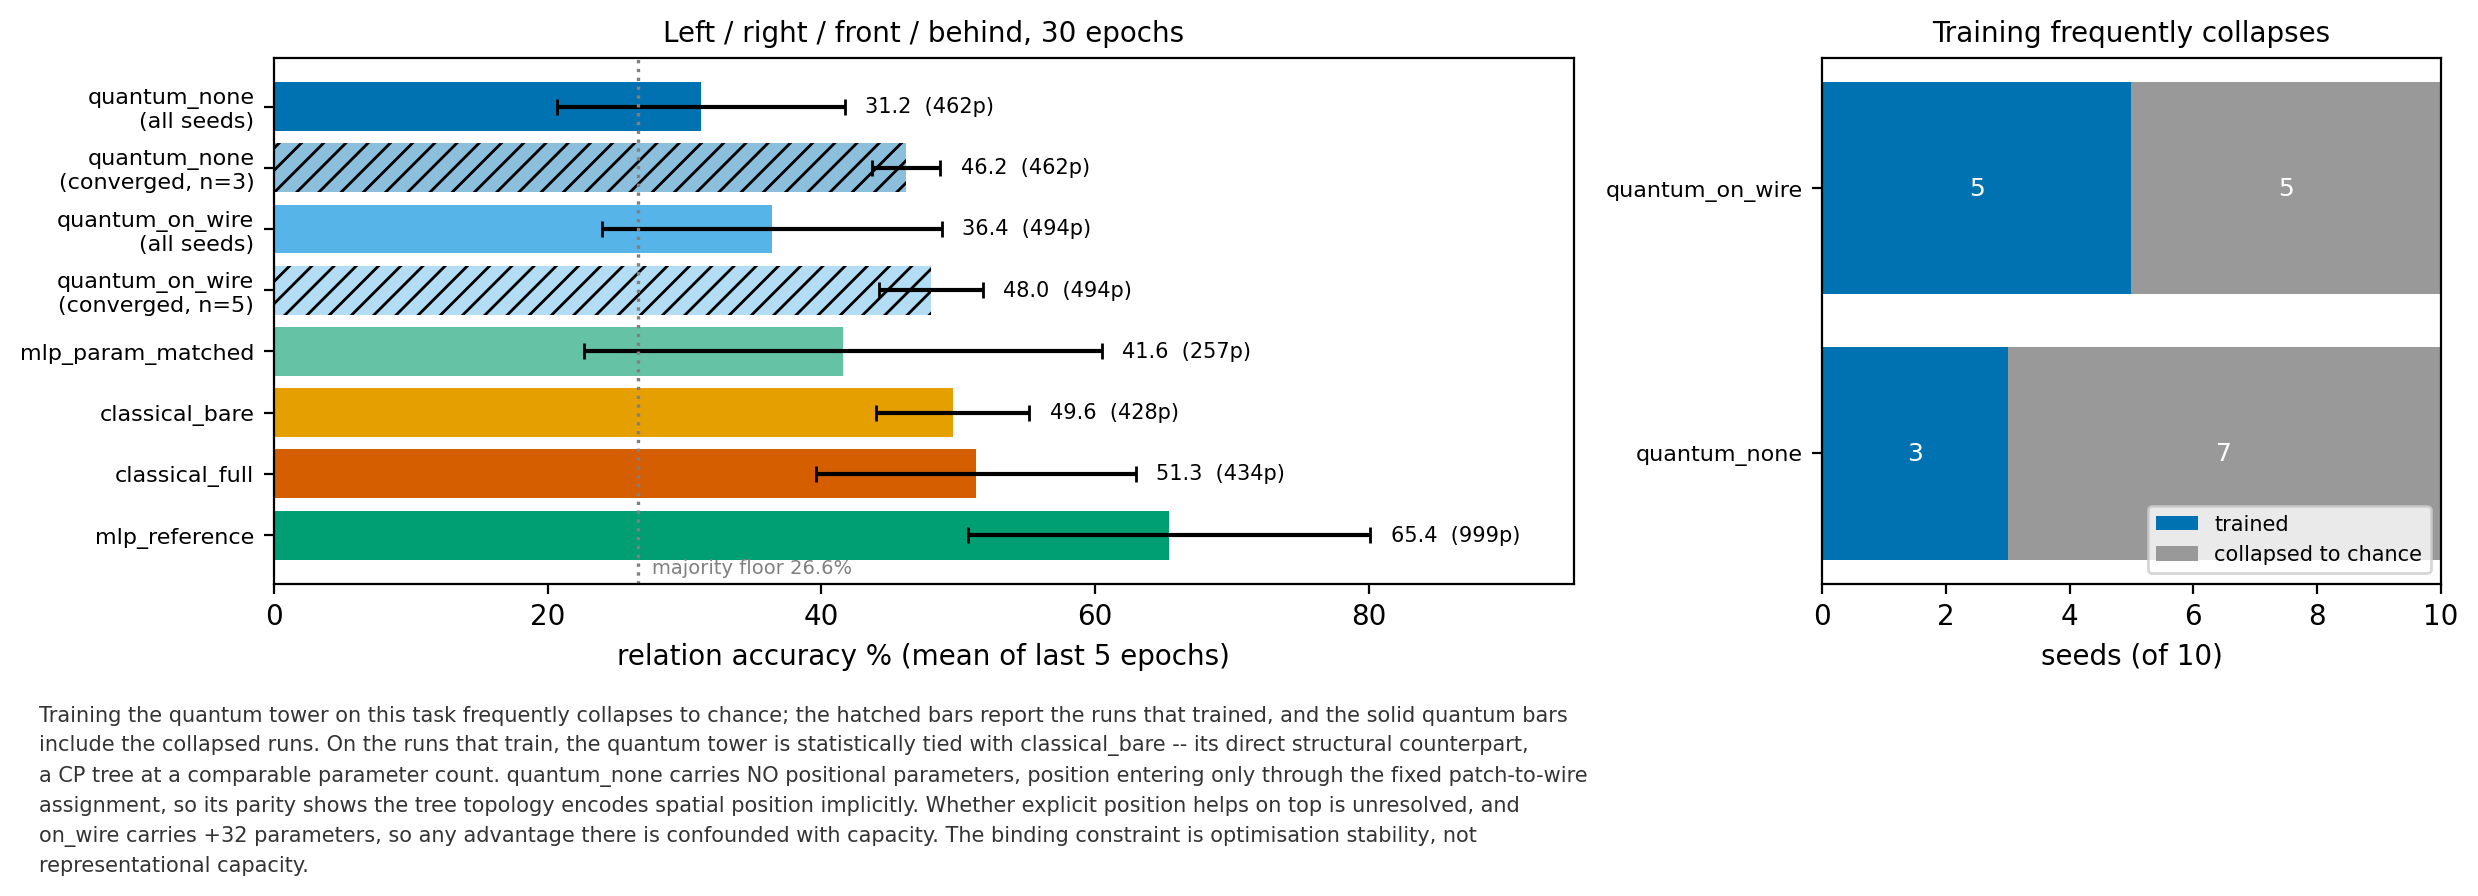
\includegraphics[width=1.0\textwidth]{ch3/clevr_relations.png}
    \caption{Relational classification. Hatched bars report the runs that trained; solid quantum bars include collapsed runs. On the runs that train, the quantum tower is statistically tied with \texttt{classical\_bare}, its direct structural counterpart at a comparable parameter count.}
    \label{fig:clevr_relations2}
\end{figure}

\section{The Compositional Binding Probe}
\label{sec:binding_probe}

While the preceding tasks established visual competency and relational geometry, neither perception nor spatial routing is inherently compositional. To probe the architectural limits that defeat contrastive Vision-Language Models, we conduct a binding probe experiment. The model is presented with two-object CLEVR composites, where each composite contains exactly one physically large object and one physically small object. The label is simply which side the large object sits on; consequently, the class-conditional marginal distributions of the raw visual features are identical by construction. The architecture must successfully bind the \texttt{size} attribute to a specific spatial coordinate to resolve the task.\footnote{The binding probe relies exclusively on the \texttt{size} attribute because the perception baseline of Table \ref{tab:perception_results} proved it is the one attribute every evaluated architecture can reliably see, at $91.8$--$98.6\%$ against a $50.6\%$ floor. A parallel binding probe using the \texttt{shape} attribute was abandoned as confounded: several baseline architectures sat at the perception floor for shape extraction, so a failure to bind shape could not be distinguished from a failure to perceive it. Binding is a conjunction of perception and binding, so only an attribute all arms perceive can isolate the second.}

Every classical architecture was evaluated against a patch-shuffled control. As detailed in Table \ref{tab:binding_results}, randomizing the spatial order of the image patches instantly collapses every one of them to exactly chance. This control mathematically guarantees that a naive "bag-of-features" model cannot solve the probe. The classical tensor networks successfully achieve this binding, resolving the task at 91.5\% and 93.2\%. However, they do not bind \emph{better} than an unstructured baseline: a 683-parameter \texttt{mlp\_param\_matched} architecture reaches 94.6\% with fewer parameters than any tensor-network arm. Because the binding task effectively saturates across all functional architectures (a 4.5-point variance across the classical spectrum), it acts as a binary diagnostic of whether an architecture binds, not how well. We can therefore state plainly that within the isolated vision tower, there is no compositional advantage for tensor networks over a plain multi-layer perceptron.

\begin{table}[hbt!]
    \centering
    \begin{tabular}{l c c c c}
        \toprule
        \textbf{Architecture} & \textbf{Params} & \textbf{Composites} & \textbf{Shuffled} & \textbf{Gap} \\
        \midrule
        \texttt{mlp\_reference}      & 1397 & $96.0 \pm 1.3$ & $50.2 \pm 2.1$ & $+45.8$ \\
        \texttt{mlp\_param\_matched} & \textbf{683}  & $94.6 \pm 2.9$ & $49.3 \pm 2.7$ & $+45.3$ \\
        \midrule
        \texttt{classical\_full}     & 942  & $93.2 \pm 1.4$ & $49.3 \pm 2.7$ & $+43.9$ \\
        \texttt{classical\_bare}     & 930  & $91.5 \pm 3.1$ & $51.0 \pm 1.4$ & $+40.5$ \\
        \midrule
        \multicolumn{5}{l}{\textit{Quantum, 15 seeds each: best seed (count $>3$ s.d. above floor)}} \\
        \texttt{quantum\_none} (implicit)  & 725 & $69.0$ \textit{(5/15)} & --- & --- \\
        \texttt{quantum\_on\_wire} (+pos.) & 757 & $73.8$ \textit{(3/15)} & --- & --- \\
        \midrule
        \textit{chance}              & ---  & $51.2$ & $51.2$ & --- \\
        \bottomrule
    \end{tabular}
    \caption{Compositional binding with class-conditional marginals equalised by construction. Every classical architecture falls to chance once patches are shuffled, so the task cannot be solved without binding an attribute to a position. Tensor networks bind; a 683-parameter MLP, smaller than any of them, binds slightly better. Quantum arms report the best seed and the count clearly above floor, since their distribution is bimodal and a mean would describe neither the capability nor the failure.}
    \label{tab:binding_results}
\end{table}

Interestingly, the 725-parameter \texttt{quantum\_none} architecture carries zero explicit positional parameters; position enters the quantum statevector solely via the fixed mapping of image patches to data wires. Despite this, the network successfully resolves the binding probe using only its topology, putting 5 of its 15 seeds more than 3 binomial standard deviations above the chance floor, peaking at 69.0\% ($8.1$ s.d.). Furthermore, explicitly injecting coordinate embeddings into the tree (\texttt{quantum\_on\_wire}) yields no statistically resolvable improvement over the implicit topology: comparing the two arms on their full distributions rather than their best runs, the gap is $-0.6$ points against an MDE of $5.5$, with both arms carrying signal. This is a bounded null rather than an absence of evidence, and it supports our previous results pointing towards the omission of explicit positional data from the quantum node.
It should be noted that the quantum models still suffer from model collapse with the majority of quantum seeds collapsing to chance. 


\section{The Frozen Baseline: CLIP's Binding Geometry}
\label{sec:clip_geometry}

We ran the same probe on a frozen CLIP image encoder \cite{radford2021learning}.
Rather than training a classifier on its features, we looked at how far its
output moves when the image changes, because comparing outputs this way,
by cosine similarity, is exactly what CLIP does when it retrieves or
classifies an image. Each comparison reuses the same two objects, so only their
arrangement differs. Swapping the two objects between sides moves CLIP's output
by $0.0050$; replacing them with different objects moves it by $0.0654$, some
thirteen times further.\footnote{Composites for this measurement are built at
CLIP's native $224 \times 224$ input resolution rather than the $32 \times 32$
used for the trainable arms, since a frozen encoder cannot be re-fit to a
smaller input. The construction is otherwise identical. The reported figures
take the \textit{jitter} condition as the reference rather than the unmodified
image, which is the conservative choice: it charges the swap only with movement
beyond what repositioning the same objects already causes.} A control confirms
that CLIP does tell these images apart, so this is not simply a failure to see
them at all. CLIP is therefore not blind to how objects are arranged, but
rearranging them registers as only $7.6\%$ of the change caused by swapping the
objects themselves. On composites built the same way, a 683-parameter network
tells the two arrangements apart $94.6\%$ of the time. This helps explain why
such models behave like bags of words on ARO \cite{yuksekgonul2023when}. The
measurement describes what CLIP's own similarity responds to, not whether the
information could be extracted by other means.



% ==========================================
% CHAPTER 6: ARO
% ==========================================
\chapter{ARO: Vision-Language Integration}
\label{ch:aro}

Having established the compositional capabilities of tensor topologies on isolated vision tasks, the final phase integrates the quad-tree architecture into a full Vision-Language Model (VLM) via the Attribution, Relation, and Order (ARO) benchmark. 

\section{Scaling Limits and the Classical Pivot}

Natural images carry far more structure than a $4 \times 4$ patch grid can represent, so transitioning to a full VLM requires deepening the quad-tree. The tower used here operates on $64 \times 64$ inputs divided into $4 \times 4$ pixel patches, giving a $16 \times 16$ grid of 256 patches and a tree of depth four rather than the depth-two, 16-patch tree of the preceding chapters.

As established in Chapter \ref{ch:theory}, the qubit count of the coherent architecture is set by the number of patches. A 256-patch grid therefore requires a 256-qubit input layer, and because physical quantum hardware is unavailable we would have to simulate it exactly, at $\mathcal{O}(2^N)$. Sixteen qubits is trivial; 256 is not merely expensive but physically impossible, exceeding the number of atoms available to store the amplitudes. The coherent quantum circuit is therefore abandoned for this final phase, and the abandonment is unconditional rather than a matter of budget.

We pivot instead to the classical CP-TTN, which preserves the hierarchical quad-tree topology exactly while contracting through unconstrained CP nodes rather than unitaries. Chapters \ref{ch:synthetic} and \ref{ch:clevr} established that the two node types are statistically tied, so this substitution changes the node's mathematical constraint without changing the structure under test. Concretely, the tower corresponds to the \texttt{classical\_full} arm rather than \texttt{classical\_bare}: it carries dropout, and residual connections on its upper two levels. This is a deliberate departure from the quantum node, which Section \ref{sec:ablations} showed is actively harmed by both mechanisms --- the classical tree, as Table \ref{tab:model_comparison} showed, depends on them.

\section{The DisCoViz Architecture}

To achieve true end-to-end compositional reasoning in a multimodal setting, we introduce DisCoViz. This architecture replaces the standard, structurally blind vision encoders utilized in traditional VLMs with our optimized Canonical Polyadic Tree Tensor Network (CP-TTN). By integrating this inherently compositional 2D vision backbone with the DisCoCat language model \cite{discocat}, DisCoViz provides a fully compositional, top-down architecture for multi-modal reasoning. 

However, integrating the hierarchical image TTN into a shared contrastive latent space alongside a text model required solving three distinct problems: preparing patches for contraction, maintaining relational capacity during that contraction, and aligning disparate multi-modal scales.

\subsection{Bilinear Patch Embedding}
Each $4 \times 4$ patch enters the tree as a bond-dimension-64 vector. Rather than flattening colour and position into a single linear map, the embedding factorises them: one learned factor contracts the three colour channels and a second contracts the sixteen pixel positions, and the two are combined by an elementwise product. This separates \textit{what} a patch contains from \textit{where} within the patch it sits, and the multiplicative combination lets the two interact without either dominating the other at initialisation.

\subsection{The Inverted Funnel}
To mitigate severe information bottlenecks during spatial contraction, the TTN vision backbone utilizes an "Inverted Funnel" structure. In a standard hierarchical network, compressing the spatial resolution inherently risks destroying fine-grained relational data. To prevent this, the internal bond dimension ($D$) of the TTN explicitly expands at each depth level, doubling as the spatial resolution is reduced by a factor of four ($D_{out} = 2 \times D_{in}$).

This structural expansion provides the "expressive headroom" necessary to encode complex multi-linear interactions. The $16 \times 16$ grid of 256 patches contracts over four levels --- 256 patches to 64, then 16, then 4, then a single root --- while the bond dimension runs $64 \to 128 \to 256 \to 512 \to 1024$. The root tensor is therefore 1024-dimensional, and a final linear projection maps it to the 512-dimensional embedding shared with the text tower. The increasing dimensionality ensures that critical spatial relationships are preserved rather than destructively pooled.

\subsection{Positional Encoding}
The vision tower carries a learned positional embedding, one vector per patch, added to the patch representations before contraction and scaled by a learned gate initialised to a small fraction of the signal. This is a departure from the quantum tower of Chapters \ref{ch:synthetic} and \ref{ch:clevr}, where explicit positional parameters were shown to be unnecessary --- the tree's fixed patch-to-wire assignment supplied position implicitly, and adding an explicit mechanism yielded no resolvable benefit.

That earlier result was a bounded null rather than a demonstration that positional encoding is harmful, and it was measured on a depth-two tree over 16 patches. At depth four over 256 patches the implicit signal is considerably weaker: a patch's identity must survive four contractions rather than two, and the number of positions it must be distinguished from is sixteen times larger. The gating is what makes the addition safe --- initialised small, the network is free to leave the positional signal near zero if the implicit topology already suffices. Whether it is in fact needed at this depth was not measured, and is a natural extension of the Chapter \ref{ch:clevr} ablation to the scaled architecture.

\subsection{Output Normalization}
A critical observation during the initial integration phase was a severe scale mismatch between the outputs of the two modalities. The raw mathematical norms of the TTN image embeddings and the DisCoCat text embeddings differed by several orders of magnitude. This scale discrepancy heavily destabilized the contrastive gradients and rendered cosine-based similarity metrics ineffective, causing early training attempts to stagnate.

To resolve this, we implemented explicit L2-normalization at the final projection head of both network towers. This standard operation normalizes the final image and text embeddings to unit length, ensuring they reside on a shared unit hypersphere. This geometric alignment provided the mathematical stability required for the contrastive loss function to effectively train the model on fine-grained compositional tasks.

\section{The ARO Dataset and Setup}

To evaluate DisCoViz, we utilized the Attribution, Relation, and Order (ARO) benchmark. ARO exposes the "bag-of-features" vulnerabilities in standard VLMs by challenging them to distinguish true captions from structurally swapped hard negatives. We evaluate on two specific tasks: \textbf{Attribution}, requiring the model to bind adjectives to specific nouns (e.g., distinguishing "a red door and a blue wall" from the hard-negative distractor "a blue door and a red wall"); and \textbf{Relation}, requiring the resolution of explicit spatial or action-based geometries (e.g., "a horse eating grass" vs. "grass eating a horse").


To optimize the network for these fine-grained distinctions, the architecture is trained using a composite loss function ($L_{total} = L_{InfoNCE} + \lambda L_{Triplet}$). The InfoNCE component maintains global latent alignment across the batch by maximizing the cosine similarity ($\text{sim}$) of matching image-text pairs $(I_i, T_i)$ against all other mismatched pairs $(I_i, T_j)$:
\begin{equation}
    L_{InfoNCE} = - \frac{1}{N} \sum_{i=1}^N \log \frac{\exp(\text{sim}(I_i, T_i) / \tau)}{\sum_{j=1}^N \exp(\text{sim}(I_i, T_j) / \tau)}
\end{equation}
where $N$ is the batch size and $\tau$ is a fixed temperature, held at $0.07$ rather than learned. A learnable temperature was tried and abandoned: it collapsed towards zero during training, sharpening the softmax until the gradient signal from all but the hardest negative vanished.
Simultaneously, the Triplet loss explicitly leverages the hard negatives provided directly by the ARO dataset. For a given anchor image $I_i$, a true caption $T_i$, and a hard-negative swapped distractor $T_{neg}$, the loss is formulated as:
\begin{equation}
    L_{Triplet} = \max(0, \text{sim}(I_i, T_{neg}) - \text{sim}(I_i, T_i) + \alpha)
\end{equation}
where $\alpha$ represents the margin. By prioritizing these hard-negative gradients through the $\lambda$ scaling factor, the optimizer is forced to mathematically resolve the subtle structural differences between the true captions and the specific shuffled distractors.

Crucially, the baseline for this evaluation is \textbf{DisCoClip} \cite{discoclip}. Both DisCoViz and DisCoClip utilize the exact same compositional DisCoCat language model for text embedding, so the language-processing capacity is held constant and any performance delta originates on the vision side. DisCoClip relies on a frozen, self-attention-based CLIP Vision Transformer, whereas DisCoViz utilizes the CP-TTN.

Two things differ between those encoders, and it is worth being precise about which one the experiment isolates. The first is architectural: global self-attention over a flattened patch sequence against hierarchical 2D contraction. The second is that CLIP's tower is \textit{frozen} while the CP-TTN is \textit{trained}. A performance delta is therefore attributable to the replacement of the encoder as a whole, and not to topology alone; separating the two would require a trained non-hierarchical tower of comparable size, which we did not run. What the comparison does establish cleanly is that the tensor-network tower is a viable substitute for frozen CLIP in a compositional setting --- which is the claim the wider programme rests on, since the motivation for replacing CLIP was never that attention is inferior in principle, but that a frozen general-purpose encoder discards the spatial information these tasks depend on, as measured directly in Section \ref{sec:clip_geometry}.

\section{Compositionality Results}

Following the architectural integration of the CP-TTN vision backbone with the DisCoCat language model, DisCoViz demonstrated exceptional compositional reasoning. On the rigorous ARO benchmark, the model achieved a 77.65\% selection accuracy on the Attribution task and a 59.78\% selection accuracy on the Relation task. 

To contextualize these results, DisCoViz was evaluated against both the direct DisCoClip baseline and industry-standard Vision-Language Models (Table \ref{tab:aro_results}).

\begin{table}[hbt!]
    \centering
    \begin{tabular}{l c c}
        \toprule
        \textbf{Architecture} & \textbf{ARO Attribution} & \textbf{ARO Relation} \\
        \midrule
        \texttt{CLIP} \cite{radford2021learning} & 61.00\% & 51.53\% \\
        \texttt{OpenCLIP} & 59.13\% & 50.71\% \\
        \texttt{BLIP} & \textbf{78.46\%} & 52.90\% \\
        \midrule
        \texttt{DisCoClip} (Baseline) & 70.01\% & 55.81\% \\
        \textbf{\texttt{DisCoViz} (Ours)} & 77.65\% & \textbf{59.78\%} \\
        \bottomrule
    \end{tabular}
    \caption{Compositional performance on the ARO benchmark. DisCoViz gains $+7.64$ and $+3.97$ points over the DisCoClip baseline, and exceeds the far larger BLIP model on the Relation task. Note that the CLIP, OpenCLIP and BLIP rows are zero-shot, whereas DisCoClip and DisCoViz are trained on the ARO training split; the rows above and below the first rule are therefore not directly comparable.}
    \label{tab:aro_results}
\end{table}

The most critical comparison is between DisCoViz and the DisCoClip baseline, since these two share both the language model and the training regime and differ only in the vision encoder. DisCoViz gains $+7.64$ points on Attribution and $+3.97$ on Relation, and both gains originate on the vision side.

The mechanism behind that gain is worth stating carefully, because Section \ref{sec:binding_probe} constrains what may be claimed. In a controlled vision-only test with the class-conditional marginals equalised by construction, tensor networks did \emph{not} bind better than a parameter-matched neural network; the binding probe saturated and ranked the two as equivalent. The improvement here is therefore not evidence that hierarchical contraction binds more effectively than the alternatives. What Section \ref{sec:clip_geometry} measured is the more likely explanation: frozen CLIP's embedding moves an order of magnitude further when the objects in a scene change than when the same objects are rearranged, so the representation DisCoClip receives has already discarded most of the arrangement information its language model would need. Replacing that encoder with any tower that preserves spatial arrangement --- and is trained to do so on this data --- recovers the discarded signal. The tensor network is a sufficient such tower, and its compositional structure makes it a natural counterpart to the compositional text model, but the result does not establish that it is the only one.

DisCoViz also exceeds CLIP and OpenCLIP by a wide margin, and exceeds BLIP on Relation ($59.78\%$ against $52.90\%$) while falling slightly short on Attribution ($77.65\%$ against $78.46\%$). These three rows are zero-shot evaluations of general-purpose models, whereas DisCoViz is trained on ARO's own training split with its hard negatives in the loss, so the comparison indicates what a small, task-adapted compositional model can achieve rather than a like-for-like architectural ranking. Read with that qualification, the relational result is the more interesting of the two: parameter scale appears to buy attribution binding, which is largely a matter of associating adjectives with nouns, more readily than it buys the geometric relationships that a structurally rigorous topology encodes directly.


% ==========================================
% CHAPTER 5
% ==========================================
\chapter{Conclusion and Future Work}

\section{Conclusion}

This report set out to build the missing half of a quantum-inspired
vision--language model. The language side already existed in DisCoCat, whose
contraction follows a sentence's grammatical structure; the open question was
whether an image encoder could be built on the same principle, and whether
replacing its classical tensor nodes with genuine quantum unitaries costs or
buys anything. We surveyed a family of candidate encoders --- tree,
matrix-product and MERA topologies across four data encodings and three
ans\"{a}tze --- narrowed them on measured evidence, and evaluated the survivor
in isolation, on CLEVR, and finally as one tower of a full vision--language
model.

\subsection{Architecture}

The selected architecture is a coherent quantum tree tensor network. Two design
decisions proved load-bearing and were each established the hard way:
intermediate states must pass between tree levels as qubits rather than being
measured and re-encoded, and the model must read its top layer rather than a
single root, the latter a consequence of a classical simulation limit rather
than a design preference. Mechanisms that classical intuition recommends, most
notably residual connections and explicit positional encoding, were tested and
rejected on positive evidence rather than dismissed on principle.

\subsection{The Quantum Node}

The unitarity constraint is not a handicap. Under matched conditions the
quantum tree node outperforms its unconstrained classical counterpart while
using roughly a third fewer parameters, and this parameter efficiency
reproduces on real data rather than holding only on synthetic benchmarks. A
secondary observation concerns multi-head training: extending the optimisation
budget causes attribute heads sharing a single loss to trade against one
another rather than improve together.

\subsection{Compositional Structure}

The aim was to establish that a quantum-native architecture can capture
compositional structure, and it does. On a probe whose class-conditional
marginals are identical by construction, validated by a control in which
every architecture falls to exactly chance under patch shuffling, so that any
above-chance score provably requires binding an attribute to a position, the
quantum tower separates the arrangements at many standard deviations above
chance. It does so in the variant carrying no positional parameters whatsoever,
with position entering only through the fixed assignment of image patches to
qubit wires. The tree's topology is therefore sufficient on its own:
compositional structure is captured by the architecture rather than supplied to
it, and adding an explicit positional mechanism changes nothing measurable.

Two boundaries belong with that result. The quantum tower reaches this solution
in a minority of initialisations, so what is established is capability rather
than reliability; and on the same probe a plain neural network of comparable
size binds equally well, so the finding is that the quantum-native route
\emph{works}, not that hierarchical contraction is the only architecture that
can. Both possibilities were registered in advance of the measurement.

\subsection{From Viability to a Vision--Language Model}

That capability matters because of where the architecture is destined. Measured
directly in the metric it uses at inference, a frozen CLIP encoder responds an
order of magnitude more strongly to which objects are present than to how they
are arranged, on images that a very small model separates almost perfectly.
Replacing that encoder with a tensor-network tower, while holding the language
model fixed, improves compositional performance on both ARO tasks and surpasses
a far larger foundation model on relational reasoning.

Taken together these results support the wider programme. The tensor-network
vision tower demonstrably improves compositional performance in a full
vision--language model; its quantum counterpart demonstrably performs the same
binding at a fraction of the parameters. A quantum-native vision--language
model is therefore a viable path rather than a speculative one, with the
qualification that the two halves of that argument have so far been measured
separately, since the quantum tower has not yet been placed in the full
pipeline.

\subsection{Limitations}

The scale at which these claims hold is narrow. A single small image size at
shallow depth is the only configuration trained end to end, and every noise
result characterises an individual tree node rather than the assembled tower.
Both are consequences of classical simulation cost rather than of the
architecture, and both, along with the training instability noted above,
are addressed in the future work that follows.


\section{Future Work}

Two directions follow from this work. The first is a set of experiments blocked
not by the architecture but by the cost of simulating it classically, which
become tractable on quantum hardware. The second is the design of a
vision--language model in which both towers, and the comparison between them,
are quantum.

\subsection{Execution on Quantum Hardware}

Several of this project's sharpest limitations are properties of the simulator
rather than of the model, and they share a signature: the technique is already
validated, and only its classical emulation is infeasible.

The clearest case is \textbf{active qubit recycling}. Measuring and resetting
qubits once a tree node has consumed them was shown to be mathematically exact,
reducing a sixteen-qubit tree to seven physical qubits with an identical output.
It does not extend beyond depth two in simulation for reasons entirely internal
to simulators: the deferred-measurement transform allocates a fresh ancilla wire
for every measurement, and the alternative branch-tracking strategy grows
exponentially in the number of resets. On hardware, mid-circuit measurement and
reset are native operations with no such blow-up, and the saving is
substantial --- a tree that would nominally require eighty qubits fits in
roughly eight. Recycling therefore converts tree depth from an unreachable
regime into a question of latency and gate error.

That in turn unlocks \textbf{training at greater depth}, the project's narrowest
constraint: one small image size at depth two is the only configuration trained
end to end. Forward passes already run at depth three and four on a
tensor-network simulator, but that device provides no backpropagation, and
gradients by parameter shift cost close to a minute per step. Parameter shift is
the native gradient method on hardware, so the very procedure that makes deeper
trees prohibitive to simulate is how they would be trained physically.

A third experiment addresses a measured defect rather than a scaling ambition.
The tower reads its top layer rather than contracting to a single root, because
reading the root alone costs more than forty accuracy points. This is a
workaround for a bond dimension of one, imposed by statevector memory: every
additional qubit per node doubles the simulated state, while on hardware the
cost is merely linear. Increasing the bond dimension would test whether the
architecture as originally designed --- a tree that genuinely contracts to a
root --- performs as intended.

Hardware would also permit two measurements currently possible only in
miniature. All noise results in this report characterise a \emph{single} tree
node, because simulating a noisy sixteen-qubit circuit requires a density matrix
of prohibitive size; on hardware noise is not emulated but inhabited, so the
resilience of the assembled tower could be measured directly. Similarly, the
gradient-scaling study stops at twenty qubits because automatic differentiation
caches a statevector at every gate, whereas sampling gradients physically would
allow the polynomial-scaling claim to be tested at widths where it becomes
falsifiable.

\paragraph{What hardware would not resolve.} The binding constraint on this
architecture is optimisation stability, and that is not a simulation artefact.
If anything, physical execution sharpens it: simulation returns exact
expectation values, whereas hardware returns sampled estimates, adding shot
noise to a landscape on which training already collapses from a substantial
fraction of initialisations.

That instability is well documented in the wider literature, and our
observations match it closely. Anschuetz and Kiani show that variational models
which are shallow and exhibit \emph{no} barren plateaus can nonetheless be
untrainable, because only a superpolynomially small fraction of their local
minima lie within any constant energy of the global optimum, rendering such
models untrainable absent a good initial guess \cite{anschuetz2022traps}. This
describes our situation precisely: gradient variance measurements confirm the
absence of a barren plateau at the widths used, yet a majority of random
initialisations never leave chance --- a landscape densely populated with traps
rather than a flat one. Consistent with this, the tensor-network-specific
analysis of Liu et al.\ finds that barren plateaus are absent for
\emph{local} loss functions, with tree tensor networks showing polynomially
decaying gradient variance, better-behaved than matrix product states
\cite{liu2022tnbp} --- again matching our measurements, and again not sufficient
for reliable training.

Two remedies from that literature are worth testing. The identity-block
initialisation of Grant et al.\ constrains the circuit to evaluate to the
identity at the start of training, bounding its effective depth on the first
update \cite{grant2019init}; we tested a near-identity variant and found no
measurable effect, which is consistent with a trap-dominated rather than
plateau-dominated landscape. More promising is \emph{warm-starting from a
classical tensor network}: Rudolph et al.\ train a matrix product state
classically, transfer it into a parametrized circuit, and report gradient
magnitudes that remain stable where randomly initialised circuits decay
exponentially, at scales up to a hundred qubits \cite{rudolph2023pretraining}.
The correspondence is unusually direct in our case, since the classical CP tree
tensor network is not an analogue of the quantum tower but its structural
counterpart, trained on the same data and already known to converge reliably. A
trained classical tree could therefore supply the quantum circuit's initial
parameters rather than random values. Related work embeds pre-trained tree
tensor networks into quantum classifiers through adiabatic encoding, removing
the postselection overhead that would otherwise make such transfers impractical
\cite{murota2025ttn}.

\subsection{Towards a Fully Quantum Vision--Language Model}

The architecture described here is quantum up to a classical boundary: patch
data is encoded into rotation angles, and measured expectation values are
projected into an embedding space where similarity is computed classically.
Those two interfaces are unavoidable for a model that consumes images and
produces scores. A more ambitious design would keep both towers as quantum
circuits and compare their outputs quantum-mechanically, never materialising an
embedding vector at all. Two problems stand between the present work and that
design, and neither is incidental.

\paragraph{The similarity measure.} Contrastive training requires a similarity
between an image representation and a text representation, and the obvious
quantum analogue of cosine similarity is state fidelity, estimated by a SWAP
test. The substitution is less direct than it appears. Fidelity returns the
\emph{squared modulus} of the overlap, which discards sign: perfectly opposed
states are indistinguishable from perfectly aligned ones. Contrastive objectives
depend on pushing negatives apart, so a measure that maps maximal dissimilarity
onto maximal similarity removes the direction the gradient should travel in.

A second difficulty is more fundamental. Thanasilp et al.\ show that quantum
kernel values concentrate exponentially in the number of qubits towards a fixed
value, so that the number of measurements required for successful training
grows exponentially and predictions on unseen inputs become independent of the
input \cite{thanasilp2024concentration}. Critically for this proposal, they
identify the \emph{fidelity kernel} as particularly vulnerable, since its
reliance on a global measurement induces exponential concentration even when the
embedding's expressibility and the entanglement of the data states are low. A
similarity built on state overlap therefore inherits a known scaling pathology
rather than merely an implementation cost.

A third difficulty is specific to this architecture. Because the tree traces out
three of every four qubits, its output is a mixed state rather than a pure one;
a SWAP test on mixed states returns the Hilbert--Schmidt inner product, whose
magnitude is bounded by the purities of the states involved, so mixedness
compresses the dynamic range independently of the content being compared. Given
that survivor states were measured well inside the Bloch sphere, this is not a
hypothetical concern.

Alternatives exist and each trades one difficulty for another. A Hadamard test
recovers the real part of the overlap and therefore preserves sign, at the cost
of a controlled operation. A small trained circuit could take both registers and
emit a score directly, avoiding a fixed metric but introducing another
variational object to optimise. And the present design --- measuring both towers
and comparing classically --- remains the baseline that any quantum similarity
must justify itself against, since it is cheap, signed, and free of
concentration effects.

\paragraph{Matching the two Hilbert spaces.} A second problem is structural, and
follows directly from what makes the language model attractive. In DisCoCat the
contraction topology is determined by the sentence's grammatical structure
rather than by a fixed layout, so different sentences induce different circuits
and, in general, different output register widths. Any similarity computed by
state overlap requires both states to inhabit the same Hilbert space. A quantum
vision--language model therefore needs a convention mapping every parse, of any
structure, onto a register of fixed width --- whether by padding to a maximum
arity, by a learned compression stage, or by constraining the admissible
diagrams. This is an architectural commitment rather than an implementation
detail, and a prerequisite for the similarity question above rather than a
consequence of it. It is also a problem the classical pipeline never had to
confront: projecting a contraction of any shape into a fixed-dimensional
embedding is trivial classically, and is precisely what the final linear layer
does.

\paragraph{The nearest experiment.} One study would strengthen this report
considerably at a fraction of that cost. The quantum tower and the
vision--language results were measured separately, the latter using the
classical tensor-network tower. Placing the quantum tower into the full pipeline
and evaluating it on the same compositional benchmark would join the two halves
of the viability argument. The obstacle is cost rather than design: contrastive
training requires three forward passes per sample, over far more data than the
classification experiments used, and at a seed budget dictated by the collapse
rate. Reducing that collapse rate --- most plausibly by the classical
warm-starting described above --- is therefore the prerequisite for the entire
programme, and the most valuable single piece of future work.




% =============================================
% 9. BIBLIOGRAPHY / REFERENCES
% =============================================
\bibliographystyle{unsrt}
\bibliography{references}

% =============================================
% 10. APPENDICES (Optional)
% =============================================
\appendix
\chapter{Synthetic Image Generation}

\label{appendix:synthetic_data}
This appendix contains the programmatic generation code for the synthetic shapes dataset used in Chapter \ref{ch:synthetic} to investigate trainability and optimize the tensor network topologies. The generator procedurally draws four primitives --- circle, square, triangle and cross --- with random spatial jitter and scale variation to prevent the models from memorizing absolute coordinate positions, plus low Gaussian channel noise.

It supports three modes, which draw on those primitives differently. \texttt{color\_only} pairs each of the four classes with a unique shape \textit{and} a unique colour, so the two attributes are perfectly correlated and either one identifies the class. \texttt{shape\_only} renders the same four shapes in greyscale, removing colour. \texttt{overlapping} decorrelates the two by building the four classes as a $2 \times 2$ design over $\{$red, green$\}\times\{$circle, square$\}$; the triangle and cross primitives are unused in this mode.

\textbf{All experiments reported in Chapter \ref{ch:synthetic} use \texttt{overlapping}}, which is the generator's default. The other two modes were used only for diagnostic runs. This matters when reading the accuracy figures: under \texttt{overlapping}, colour alone and shape alone each separate the four classes into two pairs, so either attribute in isolation caps at $50\%$, and only a model binding the two can exceed that ceiling.
\begin{figure}[hbt!]
    \centering
    % Ensure this path matches where you placed the image in your Overleaf project
    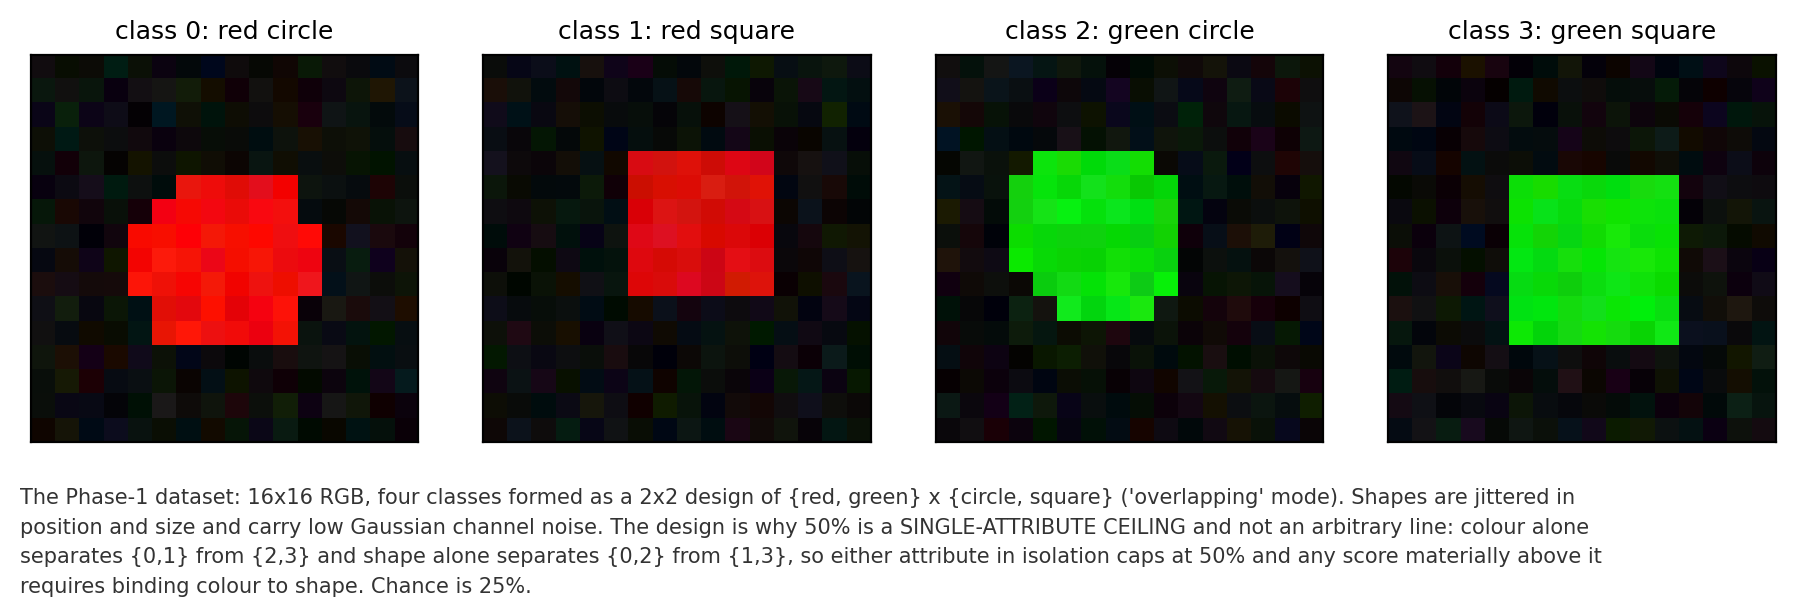
\includegraphics[width=0.8\textwidth]{ch3/synthetic_examples.png}
    \caption{Examples from the synthetic shapes dataset, illustrating spatial jitter, color variations, and geometric classes.}
    \label{fig:synthetic_examples}
\end{figure}
\section*{Code Listing: \texttt{synthetic\_shapes.py}}
\begin{minted}[
    fontsize=\footnotesize,
    frame=lines,
    breaklines,
]{python}
import numpy as np
import torch
from torch.utils.data import DataLoader, Dataset
class SyntheticShapesDataset(Dataset):
    """
    A programmatic dataset that generates 2D shape images on the fly.
    Supports three modes to test color/shape representation learning:
    - mode="color_only": Correlated unique shape/color combinations (Circle=Red, Square=Green, Triangle=Blue, Cross=Yellow).
    - mode="shape_only": Grayscale images of the 4 shapes. Color info is removed.
    - mode="overlapping": Overlapping shapes/colors (Red Circle, Red Square, Green Circle, Green Square).
    """
    def __init__(self, num_samples=1000, img_size=16, mode="overlapping", transform=None, seed=42):
        self.num_samples = num_samples
        self.img_size = img_size
        self.mode = mode
        self.transform = transform
        # Set seed for reproducibility
        self.rng = np.random.default_rng(seed)
        # Pre-generate labels so they are fixed
        self.labels = self.rng.choice(4, size=num_samples)
    def __len__(self):
        return self.num_samples
    def _draw_circle(self, grid_x, grid_y, cx, cy, r=4.0):
        return (grid_x - cx) ** 2 + (grid_y - cy) ** 2 <= r**2
    def _draw_square(self, grid_x, grid_y, cx, cy, hw=3.5):
        return (np.abs(grid_x - cx) <= hw) & (np.abs(grid_y - cy) <= hw)
    def _draw_triangle(self, grid_x, grid_y, cx, cy, h=4.0):
        # A simple upward pointing triangle
        y_cond = (grid_y >= cy - h / 2) & (grid_y <= cy + h / 2)
        x_cond = np.abs(grid_x - cx) <= (cy + h / 2 - grid_y) * 0.8
        return y_cond & x_cond
    def _draw_cross(self, grid_x, grid_y, cx, cy, l=4.0, w=1.0):
        v_bar = (np.abs(grid_x - cx) <= w) & (np.abs(grid_y - cy) <= l)
        h_bar = (np.abs(grid_y - cy) <= w) & (np.abs(grid_x - cx) <= l)
        return v_bar | h_bar
    def __getitem__(self, idx):
        label = self.labels[idx]
        # Initialize background: dark gray [0.05, 0.05, 0.05]
        img = np.zeros((3, self.img_size, self.img_size), dtype=np.float32) + 0.05
        # Create grid coordinates centered around middle of the image
        mid = (self.img_size - 1) / 2.0
        scale = self.img_size / 16.0
        # Add random spatial offset (jitter) to prevent absolute coordinate memorization
        offset_x = self.rng.uniform(-1.5, 1.5) * scale
        offset_y = self.rng.uniform(-1.5, 1.5) * scale
        cx, cy = mid + offset_x, mid + offset_y
        # Create coordinate grids
        x = np.arange(self.img_size)
        y = np.arange(self.img_size)
        grid_x, grid_y = np.meshgrid(x, y)
        # Draw the appropriate shape and assign color based on mode
        if self.mode == "color_only":
            if label == 0:  # Red Circle
                mask = self._draw_circle(grid_x, grid_y, cx, cy, r=self.rng.uniform(3.2, 4.0) * scale)
                img[0, mask] = self.rng.uniform(0.85, 1.0)
            elif label == 1:  # Green Square
                mask = self._draw_square(grid_x, grid_y, cx, cy, hw=self.rng.uniform(3.0, 3.8) * scale)
                img[1, mask] = self.rng.uniform(0.85, 1.0)
            elif label == 2:  # Blue Triangle
                mask = self._draw_triangle(grid_x, grid_y, cx, cy, h=self.rng.uniform(7.0, 8.5) * scale)
                img[2, mask] = self.rng.uniform(0.85, 1.0)
            elif label == 3:  # Yellow Cross
                mask = self._draw_cross(grid_x, grid_y, cx, cy, l=self.rng.uniform(3.5, 4.5) * scale, w=0.8 * scale)
                img[0, mask] = self.rng.uniform(0.85, 1.0)
                img[1, mask] = self.rng.uniform(0.85, 1.0)
        elif self.mode == "shape_only":
            val = self.rng.uniform(0.85, 1.0)
            if label == 0:  # Circle
                mask = self._draw_circle(grid_x, grid_y, cx, cy, r=self.rng.uniform(3.2, 4.0) * scale)
            elif label == 1:  # Square
                mask = self._draw_square(grid_x, grid_y, cx, cy, hw=self.rng.uniform(3.0, 3.8) * scale)
            elif label == 2:  # Triangle
                mask = self._draw_triangle(grid_x, grid_y, cx, cy, h=self.rng.uniform(7.0, 8.5) * scale)
            elif label == 3:  # Cross
                mask = self._draw_cross(grid_x, grid_y, cx, cy, l=self.rng.uniform(3.5, 4.5) * scale, w=0.8 * scale)
            img[:, mask] = val  # Grayscale (White)
        elif self.mode == "overlapping":
            # Shape Selection
            if label in [0, 2]:  # Circle
                mask = self._draw_circle(grid_x, grid_y, cx, cy, r=self.rng.uniform(3.2, 4.0) * scale)
            else:  # Square
                mask = self._draw_square(grid_x, grid_y, cx, cy, hw=self.rng.uniform(3.0, 3.8) * scale)
            # Color Selection
            if label in [0, 1]:  # Red
                img[0, mask] = self.rng.uniform(0.85, 1.0)
            else:  # Green
                img[1, mask] = self.rng.uniform(0.85, 1.0)
        # Add tiny Gaussian noise to represent real-world channel fluctuations
        noise = self.rng.normal(0, 0.03, size=img.shape).astype(np.float32)
        img = np.clip(img + noise, 0.0, 1.0)
        # Convert to torch tensor
        img_tensor = torch.tensor(img)
        if self.transform:
            img_tensor = self.transform(img_tensor)
        return img_tensor, torch.tensor(label, dtype=torch.long)
def get_synthetic_shapes_loaders(
    batch_size=64, train_samples=1000, test_samples=200, img_size=16, mode="overlapping", seed=42
):
    """
    Returns train and test dataloaders for the synthetic shapes dataset.
    """
    train_dataset = SyntheticShapesDataset(num_samples=train_samples, img_size=img_size, mode=mode, seed=seed)
    test_dataset = SyntheticShapesDataset(num_samples=test_samples, img_size=img_size, mode=mode, seed=seed + 1000)
    train_loader = DataLoader(train_dataset, batch_size=batch_size, shuffle=True)
    test_loader = DataLoader(test_dataset, batch_size=batch_size, shuffle=False)
    return train_loader, test_loader
\end{minted}

\chapter{Model Architectures}
\label{appendix:models}

This appendix lists the model definitions referenced in the main text. The first two listings are the arms compared in Chapter \ref{ch:synthetic}: \texttt{CoherentQTTNClassifier} is the \texttt{quantum\_coherent} arm, and \texttt{ClassicalTTNClassifier} provides both the \texttt{classical\_bare} and \texttt{classical\_full} arms, which differ only by the residual and dropout flags. The third listing, \texttt{CPQuadRankLayer}, belongs to Chapter \ref{ch:aro} rather than to the synthetic study: it is the classical tensor node of the DisCoViz vision tower, and it is included here so that the two CP implementations can be compared directly.

The listings are abridged to the structurally relevant forward path. Omitted are the alternative readout and encoding branches selected by configuration, the density-matrix code paths used only for the single-node noise sweeps, and the optional positional-encoding argument threaded through the coherent tree's circuit body --- the variant reported as \texttt{quantum\_on\_wire} in Chapter \ref{ch:clevr} and used by the scaled tower of Chapter \ref{ch:aro}. What is shown is the configuration of record in each case.

\section*{Code Listing: \texttt{CoherentQTTNClassifier}}
The fully coherent 16-qubit Quantum Tree Tensor Network (QTTN) deployed in Task R7. Unlike the measure-and-re-encode hybrid used for node-level optimization, this architecture maintains quantum coherence across the entire tree, applying unitaries directly to surviving qubits until the final multi-Pauli measurement.

\begin{minted}[
    fontsize=\footnotesize,
    frame=lines,
    breaklines,
]{python}
import numpy as np
import pennylane as qml
import torch
import torch.nn as nn

def _encode_on(encoding, inputs, wires):
    """Encode patch `w` onto wire `w` for every w in `wires`."""
    for w in wires:
        if encoding == "scalar_ry":
            qml.RY(inputs[:, w, 0], wires=w)
        elif encoding == "multi_axis":
            qml.RX(inputs[:, w, 0], wires=w)
            qml.RY(inputs[:, w, 1], wires=w)
            qml.RZ(inputs[:, w, 2], wires=w)

class CoherentQTTNClassifier(nn.Module):
    """16 patches -> 4 level-1 blocks -> 1 root, as a single coherent circuit.
    
    Wire w carries patch w. Level-1 unitaries act on [0-3], [4-7], [8-11],
    [12-15]. The level-2 unitary then acts directly on the survivors [0, 4, 8, 12] 
    -- these are still entangled with their subtrees.
    """
    def __init__(
        self, readout="root_multi_pauli", encoding="multi_axis", ansatz="iqp",
        img_size=16, patch_size=4, n_classes=4, share_level1_weights=True,
    ):
        super().__init__()
        self.grid_dim = img_size // patch_size
        self.n_patches = self.grid_dim**2
        self.n_wires = self.n_patches
        
        enc_dim = 3 if encoding == "multi_axis" else 1
        self.patch_embed = nn.Linear(patch_size * patch_size * 3, enc_dim)
        
        l1_shape = (2, 4, 3) if share_level1_weights else (4, 2, 4, 3)
        self.weights_l1 = nn.Parameter(torch.randn(*l1_shape) * 0.1)
        self.weights_l2 = nn.Parameter(torch.randn(2, 4, 3) * 0.1)
        self.head = nn.Linear(12, n_classes)  # Assuming top_layer_multi_pauli

        self.l1_blocks = [[4 * b + i for i in range(4)] for b in range(4)]
        self.l2_wires = [4 * b for b in range(4)]

        def _body(inputs, w1, w2):
            _encode_on(encoding, inputs, range(self.n_wires))
            for bi, blk in enumerate(self.l1_blocks):
                _apply_ansatz(ansatz, blk, w1 if share_level1_weights else w1[bi])
            _apply_ansatz(ansatz, self.l2_wires, w2)
            
            # top_layer_multi_pauli readout
            return [qml.expval(P(w)) for w in self.l2_wires for P in (qml.PauliX, qml.PauliY, qml.PauliZ)]

        dev = qml.device("lightning.qubit", wires=self.n_wires)
        self._circuit = qml.QNode(_body, dev, interface="torch", diff_method="adjoint")

    def forward(self, x, p_noise=0.0):
        b = x.shape[0]
        ps = x.shape[-1] // self.grid_dim
        x = x.unfold(2, ps, ps).unfold(3, ps, ps)
        x = x.permute(0, 2, 3, 1, 4, 5).contiguous().view(b, self.n_patches, -1)
        angles = torch.tanh(self.patch_embed(x)) * np.pi
        
        out = self._circuit(angles, self.weights_l1, self.weights_l2)
        out = torch.stack([torch.as_tensor(o) for o in out], dim=-1).float()
        return self.head(out)
\end{minted}

\section*{Code Listing: \texttt{ClassicalTTNClassifier} (Bare \& Full)}
The classical tensor network structural analogue used for Question A.3. To ensure a capacity-matched comparison, the \texttt{classical\_bare} model is instantiated with \texttt{use\_residual=False} and \texttt{dropout\_p=0.0}. The optimized \texttt{classical\_full} baseline toggles these parameters to \texttt{True} and \texttt{0.1}, respectively.

\begin{minted}[
    fontsize=\footnotesize,
    frame=lines,
    breaklines,
]{python}
class ClassicalTTNClassifier(nn.Module):
    """Classical CP quad-tree with the same topology as the quantum QTTN.
    16 patches -> 4 level-1 nodes (4 children each) -> 1 root -> linear head.
    """
    def __init__(self, rank=8, bond_dim=2, enc_dim=3, img_size=16, patch_size=4, n_classes=4, use_residual=False, dropout_p=0.0):
        super().__init__()
        self.grid_dim = img_size // patch_size
        self.patch_embed = nn.Linear(patch_size * patch_size * 3, enc_dim)
        
        self.level1 = CPQuadRankLayer(
            num_nodes=4, in_dim=enc_dim, out_dim=bond_dim, rank=rank, 
            use_residual=use_residual, dropout_p=dropout_p
        )
        self.level2 = CPQuadRankLayer(
            num_nodes=1, in_dim=bond_dim, out_dim=bond_dim, rank=rank, 
            use_residual=use_residual, dropout_p=dropout_p
        )
        self.head = nn.Linear(bond_dim, n_classes)

    @staticmethod
    def _group_2x2(grid):
        b, h, w, d = grid.shape
        grid = grid.view(b, h // 2, 2, w // 2, 2, d)
        grid = grid.permute(0, 1, 3, 2, 4, 5).contiguous()
        return grid.view(b, (h // 2) * (w // 2), 4, d)

    def forward(self, x):
        b = x.shape[0]
        ps = x.shape[-1] // self.grid_dim
        x = x.unfold(2, ps, ps).unfold(3, ps, ps)
        x = x.permute(0, 2, 3, 1, 4, 5).contiguous().view(b, self.grid_dim**2, -1)
        feats = torch.tanh(self.patch_embed(x))
        feats = feats.view(b, self.grid_dim, self.grid_dim, -1)
        
        x1 = self._group_2x2(feats)          # [B, 4, 4, enc_dim]
        n1 = self.level1(x1)                 # [B, 4, bond_dim]
        n2 = self.level2(n1.unsqueeze(1))    # [B, 1, bond_dim]
        
        return self.head(n2.squeeze(1))
\end{minted}

\section*{Code Listing: \texttt{CPQuadRankLayer}}
The internal node mechanics for the classical tensor network, leveraging Canonical Polyadic (CP) decomposition to merge four child nodes.

\begin{minted}[
    fontsize=\footnotesize,
    frame=lines,
    breaklines,
]{python}
class CPQuadRankLayer(nn.Module):
    """Optimized Quadtree Layer with Internal Factor Normalization."""
    
    def __init__(self, num_nodes, in_dim, out_dim, rank, dropout_p=0.0, use_residual=True, gain_factor=1.0):
        super().__init__()
        self.dropout_p = dropout_p
        self.use_residual = use_residual

        self.factor_tl = nn.Parameter(torch.empty(num_nodes, rank, in_dim))
        self.factor_tr = nn.Parameter(torch.empty(num_nodes, rank, in_dim))
        self.factor_bl = nn.Parameter(torch.empty(num_nodes, rank, in_dim))
        self.factor_br = nn.Parameter(torch.empty(num_nodes, rank, in_dim))
        self.factor_out = nn.Parameter(torch.empty(num_nodes, rank, out_dim))
        self.gain = nn.Parameter(torch.full((num_nodes, 1), gain_factor))

        if use_residual:
            self.res_proj = nn.Linear(in_dim, out_dim, bias=False) if in_dim != out_dim else nn.Identity()

        with torch.no_grad():
            for f in [self.factor_tl, self.factor_tr, self.factor_bl, self.factor_br, self.factor_out]:
                nn.init.orthogonal_(f)

    def _rms_norm(self, t, eps=1e-6):
        rms = torch.sqrt(torch.mean(t**2, dim=-1, keepdim=True) + eps)
        return t / rms

    def forward(self, x):
        # 1. Project to Rank space
        p_tl = torch.einsum("bni, nri -> bnr", x[:, :, 0, :], self.factor_tl)
        p_tr = torch.einsum("bni, nri -> bnr", x[:, :, 1, :], self.factor_tr)
        p_bl = torch.einsum("bni, nri -> bnr", x[:, :, 2, :], self.factor_bl)
        p_br = torch.einsum("bni, nri -> bnr", x[:, :, 3, :], self.factor_br)

        # 2. Internal Factor RMS Norm
        p_tl, p_tr, p_bl, p_br = map(self._rms_norm, [p_tl, p_tr, p_bl, p_br])

        # 3. Multilinear Product with Gain
        merged = p_tl * p_tr * p_bl * p_br * self.gain.unsqueeze(0)

        # 4. Dropout and Output Projection
        if self.training and self.dropout_p > 0:
            merged = nn.functional.dropout(merged, p=self.dropout_p)
        out = torch.einsum("bnr, nro -> bno", merged, self.factor_out)

        # 5. Residual connection
        if self.use_residual:
            return out + self.res_proj(x.mean(dim=2))
        return out
\end{minted}

\end{document}